% AI Image Generation using Diffusion Model
% arXiv:1706.03762 계열의 논문 판면을 따르는 학위논문 본문.
% 기존 Imperial EEE 템플릿(ic_eee_thesis.cls)은 legacy/ 로 옮겨 두었음.
% 컴파일: latexmk -lualatex main.tex

\documentclass[11pt,a4paper,oneside]{report}

\usepackage{amsmath}

% 폰트: 참조 논문과 같은 Times 계열. LuaLaTeX 이므로 OpenType 로 직접 지정
\usepackage{fontspec}
\setmainfont{TeX Gyre Termes}
\usepackage{unicode-math}
\setmathfont{TeX Gyre Termes Math}

% 판면: 본문 폭을 논문처럼 좁게 잡아 한 줄 길이를 줄임
\usepackage[a4paper,left=3.2cm,right=3.2cm,top=3cm,bottom=3cm]{geometry}

\usepackage{graphicx}
\graphicspath{{imgs/}}
\usepackage{setspace}
\usepackage[font=small,labelfont=bf]{caption}
\usepackage{booktabs}
\usepackage{titlesec}
\usepackage[hidelinks]{hyperref}

% 서지: 번호식 IEEE 스타일 (참조 논문과 동일한 형태)
\usepackage[style=ieee,backend=biber]{biblatex}
\addbibresource{references.bib}

% chapters/ 안의 파일을 \chapter{Project Specification}
\label{ch1}

\section{Introduction}

This research project is centered on examining the capabilities of Denoising Diffusion Probabilistic
Model (DDPM) in the field of image generation. The focus of this study is the generation of natural
images, evaluated on two datasets of differing resolution. The first is CIFAR-10, the standard
benchmark against which diffusion models are reported, comprising $32 \times 32$ RGB images drawn
from ten object classes; retaining it allows the results obtained here to be placed alongside the
published literature. The second is CelebA, a large-scale collection of aligned face photographs,
from which a centre crop is taken and resized to $64 \times 64$. The higher resolution is included
because architectural differences between denoising networks are difficult to observe at $32 \times
32$, where the spatial extent is exhausted after only two downsampling stages; at $64 \times 64$ a
third stage becomes available and the contribution of network depth and of the skip connections is
visible both in the metrics and in the generated samples. So that the two settings remain comparable
in training cost, a 50,000-image subset of CelebA is used, matching the size of the CIFAR-10
training split. The project aims to not only develop and train a DDPM model but also to enrich the
research with comprehensive analytical work, simulations, and the development of dedicated software
tools. This approach intends to merge theoretical insights with practical applications, contributing
significantly to the understanding and advancement of generative models in digital image processing.

This project sets the generative capability of diffusion models against the established alternatives
in the field, Generative Adversarial Networks (GANs) and Variational Autoencoders (VAEs), which
Chapter~\ref{ch2} reviews. It also explores an alternative approach by combining residual learning
with the UNet backbone that is conventionally adopted for the denoising network, giving a residual
UNet (ResUNet) in which each encoder and decoder stage is constructed from residual blocks rather
than plain convolutional stacks. This investigation into different architectural frameworks is
expected to yield insightful results regarding efficiency, effectiveness, and the quality of image
generation, thus contributing to the broader discourse on machine learning architectures in
generative applications.

\subsection{Software}

This project involves the implementation of a Denoising Diffusion Probabilistic Model (DDPM) with an
emphasis on the denoising process, for which a residual UNet (ResUNet) serves as the
noise-prediction network. Training follows the standard DDPM objective: a timestep is drawn
uniformly for each example in a batch, the corresponding noisy image is formed in closed form from
the cumulative noise schedule, and the network is optimised to predict the Gaussian noise that was
added. The quantity minimised is therefore a noise-prediction error, not a reconstruction error. A
key component of the framework is the data handling routine, which caches CIFAR-10 and CelebA as
tensors at the required resolution so that an identical training loop applies to either dataset
without modification. Dedicated classes are provided for training, sampling and evaluation, and the
diffusion process is implemented separately from the denoising network so that the architecture
under test can be exchanged without altering the generative model itself. This separation is what
makes the controlled comparison of Section~\ref{sec:simulation} possible.

\subsection{Simulation}
\label{sec:simulation}

The experimental programme holds the diffusion framework fixed and varies only the denoising
network, so that any difference in performance can be attributed to the architecture rather than to
the generative model. Three networks are trained on each of the two datasets, giving six runs in
total.

\begin{itemize}
    \item \textbf{ResUNet} is the proposed network, in which every encoder and decoder stage is built from residual blocks.
    \item \textbf{Plain UNet} is identical in every respect except that the identity shortcut is removed from each block. A shortcut adds no parameters, so the two networks have exactly the same parameter count and computational cost; this comparison therefore isolates residual learning as the single variable.
    \item \textbf{DDPM UNet} is the denoising architecture of Ho et al., with four resolution stages, self-attention at $16 \times 16$ and a skip connection taken from every residual block. Its base channel width is reduced so that its parameter count falls within a few per cent of the proposed network. Without that adjustment the published configuration would be an order of magnitude larger, and any difference in quality would reflect capacity rather than design.
\end{itemize}

All six runs share the number of diffusion steps, the noise schedule, the training objective, the
optimiser and its learning rate, the number of epochs, the data augmentation and the random seed;
sampling for every model begins from the same initial noise. Evaluation is carried out on three
levels. The restoration diagnostics are computed over a thousand held-out test images at six
separate noise levels; the distribution-level metrics require a far larger sample and are computed
from 2048 images drawn through the complete reverse process for each model; and the memorisation
check compares every generated sample against the entire training set. Analysing the models under
these matched conditions is what allows patterns and variances in the diffusion process to be
attributed to the architecture, and provides the basis on which the proposed network is judged.

\subsection{Analytical Work}

The analysis reported in Chapter~\ref{ch3} follows the design set out above. Every configuration is
trained under identical conditions and evaluated by the same procedure, so that the measurements can
be compared directly; the decisions taken during development, and the corrections made when a
measurement proved to be reporting something other than what was intended, are recorded alongside
the results rather than omitted from them. Two such corrections proved substantive enough to affect
the conclusions and are documented in place: the numerical instability of the reverse process, and
the inability of the restoration measures to anticipate generative quality.

No single number captures the performance of a generative model, and the measurements reported here
fall into three groups that answer different questions. The first group asks how faithfully a
corrupted image is restored, and comprises the Structural Similarity Index Measure (SSIM) and the
Peak Signal-to-Noise Ratio (PSNR). The second asks how closely the distribution of generated images
resembles the distribution of real ones, and comprises the Fr\'echet Inception Distance (FID) and
the Inception Score (IS). The third is not a quality measure at all but a validity check: a
nearest-neighbour comparison against the training set, which establishes that the model is
generating rather than reproducing.

\begin{itemize}
    \item \textbf{Structural Similarity Index Measure} compares two images in terms of luminance,
    contrast and structural information. It requires a matched reference image, and is therefore
    applied to the reconstruction of held-out test images rather than to unconditional samples: a
    test image is corrupted to a chosen timestep and recovered in a single step, and the recovered
    image is compared with the original. A higher value indicates a more faithful restoration.

    \item \textbf{Peak Signal-to-Noise Ratio} is computed on the same pairs and reports the mean
    squared error on a logarithmic scale, in decibels. It is reported alongside SSIM because the
    two quantify different things: SSIM responds to structural agreement, PSNR to pixel-wise
    error. Where the two disagree, the disagreement is itself informative, since it indicates that
    one network is more accurate in absolute terms while the other preserves structure better.

    \item \textbf{Fr\'echet Inception Distance} quantifies the distance between the feature
    vectors of real images and generated images calculated by a pre-trained Inception network.
    Unlike the two measures above it needs no reference image, so it applies to samples drawn from
    noise and is therefore the primary measure of generative quality in this work. A lower FID
    indicates a closer match between the generated and real distributions.

    \item \textbf{Inception Score} evaluates the clarity and diversity of generated images from
    the same samples. A higher IS suggests that the model produces distinct and confidently
    classified images, although the measure is known to reward confident classification even when
    the images are not realistic, and it is therefore read alongside FID rather than on its own.

    \item \textbf{Nearest-neighbour distance} locates, for every generated sample, the closest
    image in the training set under a pixel-space $L_2$ metric. A distance on its own cannot be
    interpreted, so the same measurement is taken for held-out real images that the model never
    saw; if the generated samples are no closer to the training set than genuine unseen images
    are, there is no evidence that the model is reproducing its training data.
\end{itemize}

Negative Log-Likelihood was considered and deliberately excluded. Obtaining it for a diffusion model
requires evaluating the full variational bound rather than the simplified training objective, and
the bound is dominated by the reverse-process variances. The implementation used here follows the
original formulation in fixing those variances to the posterior values rather than learning them, so
the resulting likelihood would report a property of that fixed choice more than a property of the
denoising network under test. Reporting it would add a number without adding evidence about the
question this project asks.

Taken together the three groups support different claims. The restoration measures compare the
networks as denoisers, which is what they are trained to be; the distribution measures compare them
as generators, which is what they are ultimately for; and the memorisation check establishes that
the second claim is meaningful. Reporting all three guards against the failure mode of selecting
whichever single metric happens to favour the proposed architecture.

% \section{Notation}
% \section{Published material}
 로 부르기 위한 탐색 경로
\makeatletter
\def\input@path{{chapters/}}
\makeatother

% 구 템플릿이 쓰던 minitoc 명령. OrigSta_Copyright.tex 를 켜도 깨지지 않도록 무해화
\providecommand{\mtcaddchapter}{}

% 표제 계층: 장식 없이 굵게만. 원 템플릿의 큰 장 제목 블록을 걷어냄
\titleformat{\chapter}[hang]{\normalfont\LARGE\bfseries}{\thechapter}{0.6em}{}
\titlespacing*{\chapter}{0pt}{0pt}{18pt}
\titleformat{\section}{\normalfont\large\bfseries}{\thesection}{0.6em}{}
\titleformat{\subsection}{\normalfont\normalsize\bfseries}{\thesubsection}{0.6em}{}

\DeclareMathOperator{\diag}{diag}
\DeclareMathOperator{\vect}{vec}

\begin{document}
\singlespacing

%%%%%%%%%%%%%%%%%%%%%%%%%%%%%%%%%%%%%%%%%%%%%%%%%%%%%%%%%%%%%%%%%%%%%%%
% 표지
%%%%%%%%%%%%%%%%%%%%%%%%%%%%%%%%%%%%%%%%%%%%%%%%%%%%%%%%%%%%%%%%%%%%%%%
\begin{titlepage}
\centering
\vspace*{2.5cm}

{\LARGE\bfseries AI Image Generation using Diffusion Model\par}

\vspace{2.5cm}
{\large Lian Choi\par}
\vspace{0.3cm}
{\normalsize CID: 01704485\par}

\vspace{2cm}
{\normalsize Supervised by\par}
\vspace{0.3cm}
{\large Dr C. Ling\par}

\vspace{1.5cm}
{\normalsize Second Marker\par}
\vspace{0.3cm}
% 실제 second marker 이름으로 교체할 것. 원 템플릿에서도 비어 있던 항목
{\large Prof. A. Another\par}

\vspace{2.5cm}
{\normalsize A Thesis submitted in fulfilment of the requirements for the degree of\par}
\vspace{0.3cm}
{\normalsize\bfseries Bachelor of Engineering in Electronic and Information Engineering\par}

\vspace{2cm}
{\normalsize Department of Electrical and Electronic Engineering\par}
{\normalsize Imperial College London\par}
\vspace{0.5cm}
{\normalsize 2024\par}
\vspace{0.4cm}
% 2024 년 제출본을 2026 년에 저자가 개정했다. 자세한 내용은 개정 노트 참조
{\small\itshape Revised 2026\par}

\vfill
\end{titlepage}

%%%%%%%%%%%%%%%%%%%%%%%%%%%%%%%%%%%%%%%%%%%%%%%%%%%%%%%%%%%%%%%%%%%%%%%
% 전면부: 초록과 목차 (로마자 쪽번호)
%%%%%%%%%%%%%%%%%%%%%%%%%%%%%%%%%%%%%%%%%%%%%%%%%%%%%%%%%%%%%%%%%%%%%%%
\pagenumbering{roman}
\pagestyle{plain}

\chapter*{Abstract}
\addcontentsline{toc}{chapter}{Abstract}
Denoising Diffusion Probabilistic Models (DDPMs) have rapidly become one of the leading families of
generative models, offering a stability of training that Generative Adversarial Networks (GANs) have
historically struggled to achieve. Within a DDPM the diffusion process is fixed and the only learned
component is the network that predicts the noise added at each step, so the choice of that network
governs the quality of the images produced. This thesis asks whether combining residual learning
with the UNet backbone conventionally used for that purpose yields a measurable improvement.

A residual UNet (ResUNet) was implemented in PyTorch, in which every encoder and decoder stage is
constructed from residual blocks rather than plain convolutional stacks, and trained directly on the
standard DDPM objective. It is assessed against two baselines under matched conditions. The first
removes the identity shortcut from each block and is otherwise identical, so that the two networks
have exactly the same parameter count and the comparison isolates residual learning as the single
variable. The second is the denoising architecture of the original DDPM, with four resolution stages
and self-attention, reduced in width so that its parameter count agrees with the proposed network to
within ten per cent. All three were trained on CIFAR-10 at $32 \times 32$ and on CelebA at $64
\times 64$, sharing the diffusion schedule, the optimiser, the number of epochs and the random seed,
and sampling from the same initial noise.

The three networks were compared on restoration accuracy, measured by structural similarity and peak
signal-to-noise ratio against held-out images at six noise levels; on distribution-level quality,
measured by the Fr\'echet Inception Distance and the Inception Score over 2048 generated samples;
and on a nearest-neighbour check against the training set that found no evidence of memorisation on
either dataset.

Every configuration was trained under three random seeds. The residual shortcut lowers the
first-epoch loss in all six paired runs, by five to eleven per cent on average, but that advantage
disappears by the fifth epoch, and at convergence the restoration measures cannot separate the two
networks: the training loss leans towards the plain variant and structural similarity towards the
proposed one, both by less than half of one per cent. Generative quality separates them, on the
deeper configuration only. On CelebA the proposed network leads in every seed, by a mean of $63.31$
FID against a seed-to-seed standard deviation of about $23$; on CIFAR-10 the paired difference is
$-3.46 \pm 13.78$ with the sign changing between seeds. Two networks that denoise equally well are
therefore shown to generate images of very different quality, a discrepancy no restoration measure
anticipated. The reference architecture remains the strongest overall, leading every restoration
measure and CIFAR-10 FID at roughly $2.3$ times the training cost, and is matched only on CelebA FID
by the proposed network.

The hypothesis accordingly receives partial and conditional support: residual learning does not
improve generated image quality at two resolution stages, where it makes no detectable difference,
but at three stages it leads in every seed by a margin larger than the observed spread. Negative Log-Likelihood was excluded on the
grounds that this implementation fixes the reverse-process variances rather than learning them, and
the comparison against Variational Autoencoder and GAN baselines was not carried out.


\chapter*{Note on the 2026 Revision}
\addcontentsline{toc}{chapter}{Note on the 2026 Revision}
This thesis was submitted in 2024 in fulfilment of the requirements for the degree of Bachelor of
Engineering. The present document is a revision prepared by the author in 2026, on the author's own
initiative and outside any programme of assessment. The academic record of the original submission
is unaffected by it.

The revision was undertaken because the original implementation contained defects that invalidated
part of what was reported. The reverse process omitted the clipping of the implied estimate of
$x_0$, which is described in Section~\ref{sec:reverse-note}, and the structural similarity figures
had been computed from images whose negative pixel values were discarded on saving. Correcting both
required the experiment to be run again from the beginning.

The opportunity was taken to strengthen the experimental design rather than merely to repeat it. The
comparison now includes a control network that differs from the proposed one only in the presence of
the identity shortcut, so that residual learning is isolated as the single variable; it adds the
reference architecture of Ho et al.\ at a matched parameter budget; it is carried out on a second
dataset at twice the resolution; and every configuration is trained under three random seeds, which
established that the most striking result of the original single-run study was noise. The evaluation
was extended from training loss and structural similarity alone to include peak signal-to-noise
ratio, the Fr\'echet Inception Distance, the Inception Score and a nearest-neighbour check against
the training set. Chapters~\ref{ch1} to~\ref{ch3} and the Conclusions were rewritten around the
results these changes produced. Chapter~\ref{ch4} was added in the same revision; it applies the
remedies proposed in the Conclusions to the proposed network and measures what each contributes.


% 제출 규정상 필요하면 아래 주석을 해제할 것 (원본 템플릿에서도 꺼져 있었음)
% \input{OrigSta_Copyright.tex}

\tableofcontents

%%%%%%%%%%%%%%%%%%%%%%%%%%%%%%%%%%%%%%%%%%%%%%%%%%%%%%%%%%%%%%%%%%%%%%%
% 본문
%%%%%%%%%%%%%%%%%%%%%%%%%%%%%%%%%%%%%%%%%%%%%%%%%%%%%%%%%%%%%%%%%%%%%%%
\clearpage
\pagenumbering{arabic}

\chapter{Project Specification}
\label{ch1}

\section{Introduction}

This research project is centered on examining the capabilities of Denoising Diffusion Probabilistic
Model (DDPM) in the field of image generation. The focus of this study is the generation of natural
images, evaluated on two datasets of differing resolution. The first is CIFAR-10, the standard
benchmark against which diffusion models are reported, comprising $32 \times 32$ RGB images drawn
from ten object classes; retaining it allows the results obtained here to be placed alongside the
published literature. The second is CelebA, a large-scale collection of aligned face photographs,
from which a centre crop is taken and resized to $64 \times 64$. The higher resolution is included
because architectural differences between denoising networks are difficult to observe at $32 \times
32$, where the spatial extent is exhausted after only two downsampling stages; at $64 \times 64$ a
third stage becomes available and the contribution of network depth and of the skip connections is
visible both in the metrics and in the generated samples. So that the two settings remain comparable
in training cost, a 50,000-image subset of CelebA is used, matching the size of the CIFAR-10
training split. The project aims to not only develop and train a DDPM model but also to enrich the
research with comprehensive analytical work, simulations, and the development of dedicated software
tools. This approach intends to merge theoretical insights with practical applications, contributing
significantly to the understanding and advancement of generative models in digital image processing.

This project sets the generative capability of diffusion models against the established alternatives
in the field, Generative Adversarial Networks (GANs) and Variational Autoencoders (VAEs), which
Chapter~\ref{ch2} reviews. It also explores an alternative approach by combining residual learning
with the UNet backbone that is conventionally adopted for the denoising network, giving a residual
UNet (ResUNet) in which each encoder and decoder stage is constructed from residual blocks rather
than plain convolutional stacks. This investigation into different architectural frameworks is
expected to yield insightful results regarding efficiency, effectiveness, and the quality of image
generation, thus contributing to the broader discourse on machine learning architectures in
generative applications.

\subsection{Software}

This project involves the implementation of a Denoising Diffusion Probabilistic Model (DDPM) with an
emphasis on the denoising process, for which a residual UNet (ResUNet) serves as the
noise-prediction network. Training follows the standard DDPM objective: a timestep is drawn
uniformly for each example in a batch, the corresponding noisy image is formed in closed form from
the cumulative noise schedule, and the network is optimised to predict the Gaussian noise that was
added. The quantity minimised is therefore a noise-prediction error, not a reconstruction error. A
key component of the framework is the data handling routine, which caches CIFAR-10 and CelebA as
tensors at the required resolution so that an identical training loop applies to either dataset
without modification. Dedicated classes are provided for training, sampling and evaluation, and the
diffusion process is implemented separately from the denoising network so that the architecture
under test can be exchanged without altering the generative model itself. This separation is what
makes the controlled comparison of Section~\ref{sec:simulation} possible.

\subsection{Simulation}
\label{sec:simulation}

The experimental programme holds the diffusion framework fixed and varies only the denoising
network, so that any difference in performance can be attributed to the architecture rather than to
the generative model. Three networks are trained on each of the two datasets, giving six runs in
total.

\begin{itemize}
    \item \textbf{ResUNet} is the proposed network, in which every encoder and decoder stage is built from residual blocks.
    \item \textbf{Plain UNet} is identical in every respect except that the identity shortcut is removed from each block. A shortcut adds no parameters, so the two networks have exactly the same parameter count and computational cost; this comparison therefore isolates residual learning as the single variable.
    \item \textbf{DDPM UNet} is the denoising architecture of Ho et al., with four resolution stages, self-attention at $16 \times 16$ and a skip connection taken from every residual block. Its base channel width is reduced so that its parameter count falls within a few per cent of the proposed network. Without that adjustment the published configuration would be an order of magnitude larger, and any difference in quality would reflect capacity rather than design.
\end{itemize}

All six runs share the number of diffusion steps, the noise schedule, the training objective, the
optimiser and its learning rate, the number of epochs, the data augmentation and the random seed;
sampling for every model begins from the same initial noise. Evaluation is carried out on three
levels. The restoration diagnostics are computed over a thousand held-out test images at six
separate noise levels; the distribution-level metrics require a far larger sample and are computed
from 2048 images drawn through the complete reverse process for each model; and the memorisation
check compares every generated sample against the entire training set. Analysing the models under
these matched conditions is what allows patterns and variances in the diffusion process to be
attributed to the architecture, and provides the basis on which the proposed network is judged.

\subsection{Analytical Work}

The analysis reported in Chapter~\ref{ch3} follows the design set out above. Every configuration is
trained under identical conditions and evaluated by the same procedure, so that the measurements can
be compared directly; the decisions taken during development, and the corrections made when a
measurement proved to be reporting something other than what was intended, are recorded alongside
the results rather than omitted from them. Two such corrections proved substantive enough to affect
the conclusions and are documented in place: the numerical instability of the reverse process, and
the inability of the restoration measures to anticipate generative quality.

No single number captures the performance of a generative model, and the measurements reported here
fall into three groups that answer different questions. The first group asks how faithfully a
corrupted image is restored, and comprises the Structural Similarity Index Measure (SSIM) and the
Peak Signal-to-Noise Ratio (PSNR). The second asks how closely the distribution of generated images
resembles the distribution of real ones, and comprises the Fr\'echet Inception Distance (FID) and
the Inception Score (IS). The third is not a quality measure at all but a validity check: a
nearest-neighbour comparison against the training set, which establishes that the model is
generating rather than reproducing.

\begin{itemize}
    \item \textbf{Structural Similarity Index Measure} compares two images in terms of luminance,
    contrast and structural information. It requires a matched reference image, and is therefore
    applied to the reconstruction of held-out test images rather than to unconditional samples: a
    test image is corrupted to a chosen timestep and recovered in a single step, and the recovered
    image is compared with the original. A higher value indicates a more faithful restoration.

    \item \textbf{Peak Signal-to-Noise Ratio} is computed on the same pairs and reports the mean
    squared error on a logarithmic scale, in decibels. It is reported alongside SSIM because the
    two quantify different things: SSIM responds to structural agreement, PSNR to pixel-wise
    error. Where the two disagree, the disagreement is itself informative, since it indicates that
    one network is more accurate in absolute terms while the other preserves structure better.

    \item \textbf{Fr\'echet Inception Distance} quantifies the distance between the feature
    vectors of real images and generated images calculated by a pre-trained Inception network.
    Unlike the two measures above it needs no reference image, so it applies to samples drawn from
    noise and is therefore the primary measure of generative quality in this work. A lower FID
    indicates a closer match between the generated and real distributions.

    \item \textbf{Inception Score} evaluates the clarity and diversity of generated images from
    the same samples. A higher IS suggests that the model produces distinct and confidently
    classified images, although the measure is known to reward confident classification even when
    the images are not realistic, and it is therefore read alongside FID rather than on its own.

    \item \textbf{Nearest-neighbour distance} locates, for every generated sample, the closest
    image in the training set under a pixel-space $L_2$ metric. A distance on its own cannot be
    interpreted, so the same measurement is taken for held-out real images that the model never
    saw; if the generated samples are no closer to the training set than genuine unseen images
    are, there is no evidence that the model is reproducing its training data.
\end{itemize}

Negative Log-Likelihood was considered and deliberately excluded. Obtaining it for a diffusion model
requires evaluating the full variational bound rather than the simplified training objective, and
the bound is dominated by the reverse-process variances. The implementation used here follows the
original formulation in fixing those variances to the posterior values rather than learning them, so
the resulting likelihood would report a property of that fixed choice more than a property of the
denoising network under test. Reporting it would add a number without adding evidence about the
question this project asks.

Taken together the three groups support different claims. The restoration measures compare the
networks as denoisers, which is what they are trained to be; the distribution measures compare them
as generators, which is what they are ultimately for; and the memorisation check establishes that
the second claim is meaningful. Reporting all three guards against the failure mode of selecting
whichever single metric happens to favour the proposed architecture.

% \section{Notation}
% \section{Published material}

\chapter{Background}
\label{ch2}


\section{Review of Literature}

Diffusion probabilistic models have emerged as a powerful class of generative models that have significantly advanced the field of image generation. These models operate by gradually transforming a distribution of random noise into a distribution of structured images over many iterative steps, effectively reversing the diffusion process. This methodology allows for the generation of highly detailed and coherent images across a range of domains and applications.

One of the most notable achievements of diffusion probabilistic models is their ability to produce images that rival the quality of those generated by other leading techniques, such as Generative Adversarial Networks (GANs). Dhariwal and Nichol report that a diffusion model surpasses the strongest available adversarial baseline on ImageNet synthesis at several resolutions \parencite{arXiv:2105.05233}, and attribute the margin to fidelity and coverage of the data distribution rather than to sample sharpness alone.

In terms of specific accomplishments, diffusion models have excelled in tasks such as high-resolution image synthesis, text-to-image generation, and image-to-image translation. For instance, they have been successfully applied to create photorealistic images of landscapes and portraits from textual descriptions, showcasing their versatility and robustness. Additionally, these models have proven capable of handling complex conditioning information, making them particularly useful for tasks requiring detailed customization of the generated content.

The theoretical underpinnings of diffusion models also contribute to their appeal. Unlike GANs, which can be challenging to train due to issues like mode collapse, diffusion models offer a more stable training process. This stability stems from their foundation in well-understood stochastic differential equations, providing a clear pathway for systematic improvements and adaptations.

\begin{figure}
    \centering
    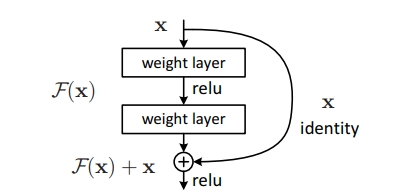
\includegraphics[width=0.5\linewidth]{imgs/Residual_learning.jpeg}
    \caption{Residual Learning: a building block \cite{arXiv:1512.03385}}
    \label{fig:residual-block}
\end{figure}

The ResNet architecture, short for Residual Network, was introduced by He et al.\ in ``Deep Residual Learning for Image Recognition'' \parencite{arXiv:1512.03385} and has since been adopted across a wide range of computer vision tasks.

ResNet’s primary innovation lies in its use of residual blocks (Figure~\ref{fig:residual-block}). These blocks allow the network to skip one or more layers through the use of shortcut connections, or skip connections, that perform identity mapping. By adding the output from an earlier layer to a later layer, these connections help to mitigate the vanishing gradient problem that plagues deep neural networks. As a result, ResNet can effectively train much deeper networks than was previously possible.

The standard implementations of ResNet include variants with different depths, typically ranging from 18 layers to 152 layers. ResNet-50, ResNet-101, and ResNet-152 are among the most popular configurations, with the number indicating the count of layers. These models are established baselines for image classification, detection and segmentation on ImageNet and COCO.

ResNet reduced classification error substantially relative to the plain architectures that preceded it, and ResNet-50 and ResNet-101 in particular are widely used because they balance depth against computational cost.

The architecture has also been applied outside image recognition, including in audio signal processing and reinforcement learning, which indicates that the benefit of residual connections is not specific to the visual domain.

Training diffusion probabilistic models presents a unique set of challenges that are both computational and theoretical in nature. These models operate by learning to reverse a diffusion process, gradually converting random noise into a structured data distribution over many iterative steps. While the results can be impressive, achieving them is far from straightforward.

One of the most significant hurdles in training diffusion models is their high computational cost. Each training iteration involves simulating the reverse diffusion process across multiple timesteps, which can be computationally intensive especially as the number of timesteps increases. This makes training such models resource-heavy, requiring powerful hardware and often resulting in long training times. Researchers have explored methods such as subsampling timesteps during training to reduce computational overhead. This approach is discussed in ``Improved Denoising Diffusion Probabilistic Models'' by Alex Nichol and Prafulla Dhariwal \cite{arXiv:2102.09672}, where they introduce techniques to selectively skip timesteps without compromising the model’s performance. 

The performance of diffusion models heavily relies on the precise tuning of hyperparameters, including the learning rate, the number of diffusion steps, and the noise schedule. Determining the optimal settings for these parameters can be a trial-and-error process that requires extensive experimentation and computational resources.

Although diffusion models are generally more stable during training compared to other generative models like GANs, they are not completely free from stability issues. Problems can arise from numerical instabilities during the simulation of the reverse diffusion process, particularly when dealing with very low probability events in high-dimensional spaces.

Diffusion models are often applied to high-dimensional data such as images, which can complicate the training process. The curse of dimensionality can exacerbate the challenges in modeling the data distribution accurately, requiring more sophisticated techniques and deeper networks. Techniques such as principal component analysis (PCA) and autoencoders have been used to reduce the dimensionality of data before training diffusion models. This can simplify the learning process and improve the manageability of high-dimensional data.

Measuring the performance of diffusion models can also be challenging. Traditional metrics like log-likelihood are not always informative for image quality in visual tasks. Alternatives like Inception Score or Fréchet Inception Distance are commonly used, but they have their limitations and may not fully capture the model’s capabilities in generating diverse and realistic images.

A practical challenge in training diffusion models for image generation is balancing the level of detail in the generated images with the diversity of the output. Overtraining on specific features can lead to loss of diversity (mode collapse), while too much randomness can reduce the realism of the generated images.

Despite these challenges, diffusion models are continuously being refined and improved, making them increasingly viable for a range of applications. Advances in computational resources, algorithmic optimizations, and better understanding of the underlying processes are helping to mitigate these difficulties, broadening the practical use of diffusion models in the field of generative modeling.

Exploring Stochastic Differential Equations (SDEs) as a modeling approach for the diffusion process has become a significant area of research in the development of diffusion probabilistic models. SDEs are used to provide a mathematical framework for modeling the continuous dynamics of the random variables involved in the diffusion process. This approach has several advantages, particularly in terms of flexibility, precision, and the ability to model complex stochastic behaviors.

Stochastic Differential Equations are used to model systems that exhibit random behavior and are influenced by continuous stochastic noise. In the context of diffusion models, SDEs describe how an image (or another data type) gradually transitions from a meaningful configuration to a state of pure noise—and vice versa—over continuous time. This is fundamentally different from the discrete step-wise approach seen in earlier diffusion models, where the process was modeled as a sequence of discrete steps.

In diffusion probabilistic models, the forward process is modeled as adding noise over time until the data becomes indistinguishable from Gaussian noise. The reverse process, which is of primary interest, involves learning the reverse of this noise-adding process. By employing SDEs, researchers can model this reverse process more naturally and fluidly as it provides a continuous-time framework, which can capture the nuances of the noise reduction at any point in time.

SDEs allow the diffusion process to be defined in continuous time, giving a finer control over the dynamics of the process. This can lead to more precise and controlled generation of the data, as the model can potentially make adjustments at any moment in the continuous timeline. The use of SDEs enables the modeling of more complex dynamics that cannot be captured by simple discrete transitions. This is particularly useful in applications where the data exhibits intricate stochastic behaviors. It is also possible to implement more efficient sampling algorithms that leverage the continuous nature of the process. For instance, adaptive step-size solvers can be used to speed up the reverse diffusion process without loss of quality.

\begin{figure}
    \centering
    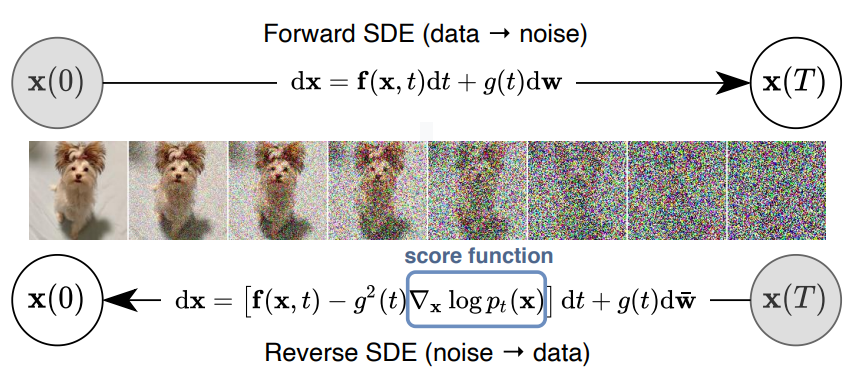
\includegraphics[width=0.5\linewidth]{imgs/Solving_a_reverse-time_SDE.png}
    \caption{Solving a reverse time SDE yields a score-based generative model. Transforming data to a simple noise distribution can be accomplished with a continuous-time SDE. This SDE can be reversed if we know the score of the distribution at each intermediate time step \parencite{arXiv:2011.13456}}
    \label{fig:reverse-sde}
\end{figure}

The seminal work by Yang Song et al. in their paper ``Score-Based Generative Modeling through Stochastic Differential Equations'' published at ICLR 2021 \parencite{arXiv:2011.13456}, is a notable contribution to this area, and the correspondence between the forward and reverse-time processes that it formalises is illustrated in Figure~\ref{fig:reverse-sde}. They propose a framework that uses score-based methods and SDEs to generate samples. By defining the generative model as a solution to an SDE, they are able to leverage the properties of differential equations to model the diffusion process more robustly and efficiently.

Despite the advantages, implementing SDEs in diffusion models also introduces new challenges. The primary issue is the computational cost associated with solving SDEs, especially in high-dimensional spaces typical of image data. Additionally, designing and training models to solve these equations requires sophisticated techniques and a deep understanding of both the theoretical and practical aspects of stochastic calculus.

\section{Analysis of Competing Products}

Denoising Diffusion Probabilistic Models (DDPMs), Variational Autoencoders (VAEs), and Generative Adversarial Networks (GANs) are all prominent types of generative models, each with unique strengths and applications.

\subsection{Variational Autoencoders (VAE)}

Variational Autoencoders (VAEs) have been a significant part of the generative modeling landscape since their introduction by Kingma and Welling in ``Auto-Encoding Variational Bayes'' \parencite{arXiv:1312.6114}. VAEs are especially valued for their robustness in learning latent representations and their ability to generate new data points with variations that are meaningful in a learned latent space.

VAEs are particularly celebrated for their ability to learn well-structured latent spaces. This means that similar data points result in close points in the latent space, making these models excellent for tasks that involve data interpolation, anomaly detection, and more. This has been critical for advancements in fields like bioinformatics where understanding the underlying structure of data is crucial.

Early criticisms of VAEs focused on their tendency to produce blurrier samples compared to GANs. However, advancements have been made to address this issue. Techniques such as using hierarchical latent variables, improving the variational bound, or incorporating better decoder architectures have significantly enhanced the quality of the generated samples. For instance, the introduction of VQ-VAE (Vector Quantized VAE) by van den Oord et al. \parencite{arXiv:1711.00937} and its successor VQ-VAE-2 by Razavi et al. \parencite{arXiv:1906.00446} showcases substantial improvements in the fidelity and diversity of generated images.

VAEs have found applications in a variety of fields beyond just image generation. In drug discovery, VAEs are used to generate novel molecular structures by learning from known chemical compounds. Similarly, in finance, they help in modeling complex financial instruments and in risk management by understanding the distributions of various financial parameters. These applications benefit from VAEs' ability to model complex, high-dimensional data in a compressed, interpretable format.

The flexibility of VAEs allows them to be effectively combined with other neural network architectures, enhancing their utility and performance. For example, the integration of VAEs with Recurrent Neural Networks (RNNs) has led to improved models for sequence data, which is useful in natural language processing and sequential image analysis.

The theoretical aspects of VAEs have also been extensively explored, leading to a deeper understanding and better implementations. Innovations such as the $\beta$-VAE, introduced by Higgins et al. \parencite{higgins2017betavae}, offer a way to balance latent channel capacity and independence constraints to control the disentanglement of latent representations, enhancing both interpretability and control over generative models.

\subsection{Generative Adversarial Networks (GAN)}

Generative Adversarial Networks (GANs) reshaped generative modelling after their introduction by Goodfellow et al.\ \parencite{arXiv:1406.2661}. The unique adversarial training approach of GANs, involving a duel between a generator and a discriminator, has led to substantial advancements in generating high-fidelity and realistic images. The achievements of GANs span various domains, from art creation to medical image analysis. 

The principal achievement of GANs is the visual quality of their samples. BigGAN \parencite{arXiv:1809.11096} and StyleGAN \parencite{arXiv:1812.04948} generate images at resolutions and levels of detail that earlier generative models did not reach, and StyleGAN in particular separates the factors of variation across its layers, so that attributes of the generated image can be controlled independently.

GANs have been successfully applied to a wide range of applications. In the field of fashion, GANs are used for creating new clothing designs and for virtual try-ons. In video games and virtual reality, they help generate realistic environments and characters. Additionally, GANs have made significant impacts in the medical field, where they are used for data augmentation in medical imaging and for generating synthetic patient data that can be used for training other AI models without privacy concerns.

GANs have also been pivotal in advancing unsupervised and semi-supervised learning techniques. The ability of GANs to learn complex distributions without extensive labeled data has made them valuable for scenarios where labeled data is scarce or expensive to obtain. For instance, models like the Semi-Supervised GAN (SGAN) \parencite{arXiv:1606.01583} leverage this capability to improve learning efficiency and accuracy using smaller amounts of labeled data supplemented with larger amounts of unlabeled data.

Despite their potential, GANs were initially known for being difficult to train, with issues such as mode collapse and non-convergence. Over the years, researchers have proposed various techniques to stabilize GAN training, such as introducing new architectures, loss functions, and regularization techniques. The introduction of the Wasserstein GAN (WGAN) \parencite{arXiv:1701.07875} marks a significant development in this area, addressing the issue of training stability through a novel loss function that provides a smoother gradient.

Analysis of the training dynamics, and in particular of how the generator and discriminator interact over the course of optimisation, has informed the architectural and loss-function changes described above.

\section{Specification of Software Standards}

\begin{itemize}
    \item \textbf{Google Python Style Guide} is a comprehensive set of guidelines that Google provides to maintain a consistent and high-quality codebase across its Python projects.
    \item \textbf{NumPy} is a fundamental library for scientific computing in Python, providing support for large, multi-dimensional arrays and matrices, along with a large collection of high-level mathematical functions to operate on these arrays.
    \item \textbf{PyTorch} is an open-source machine learning library developed by Facebook, known for its flexibility and ease of use in building and training deep learning models, particularly popular for research and prototyping.    
\end{itemize}

\section{ResNet Background Theory}

Residual Networks represent a seminal advancement in deep learning that emerged to address the vanishing gradient problem occurring in very deep neural networks. ResNet fundamentally altered approaches to network architecture design, enabling the training of networks that are substantially deeper than those previously feasible. This development has had profound implications for the field of computer vision and beyond. 

Before ResNet, increasing network depth to improve performance had reached a bottleneck. Typically, deeper networks begin to suffer from the vanishing gradient problem—where gradients become too small to make meaningful adjustments in weights during backpropagation—leading to saturation and then rapid degradation of training accuracy. Moreover, deeper networks often encounter a complexity that makes them computationally expensive and harder to optimize.

ResNet introduced a novel solution to these issues through the use of residual learning. The central hypothesis was that if deeper networks are approximations of shallower ones, then it should be easier to optimize the residual mappings rather than the desired underlying mapping.

The core idea behind ResNet is the introduction of the residual block, which includes shortcut connections (also known as skip connections). These connections allow the input to a layer to be added to its output, effectively forming an identity mapping that skips one or more layers. Mathematically, if $H(x)$ is an underlying mapping to be learned by a few stacked layers, and $x$ is the input, then these layers in ResNet fit another mapping of \eqref{eq:residual-function}. The original function thus becomes \eqref{eq:residual-identity}.

\begin{equation}
    F(x) := H(x) - x \label{eq:residual-function}
\end{equation}

\begin{equation}
    H(x) = F(x) + x \label{eq:residual-identity}
\end{equation}

This setup makes it easier to optimize the network because learning the residual mapping $F(x)$ is simpler than learning the unreferenced mapping $H(x)$. In practice, this means that even very deep networks can be trained directly through standard backpropagation. This approach addresses both the degradation problem—ensuring that adding more layers does not lead to higher training error—and reduces the impact of the vanishing gradients by providing an alternative pathway for gradient flow during backpropagation.

\begin{figure}
    \centering
    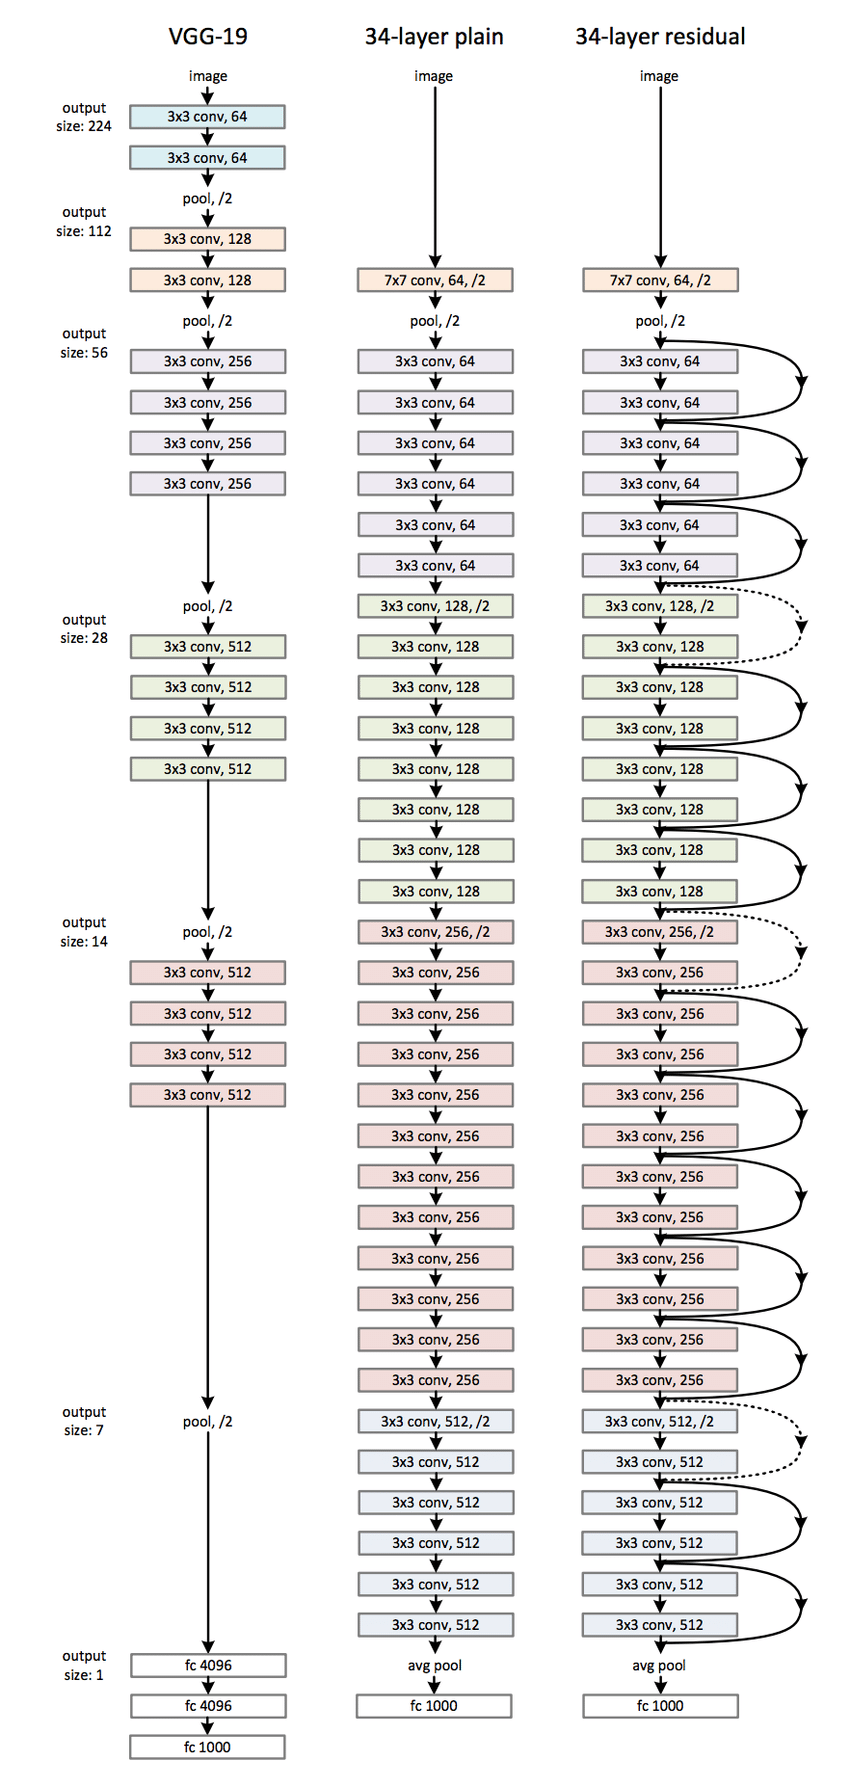
\includegraphics[width=0.5\linewidth]{imgs/Example-network-architectures-for-ImageNet-Left-the-VGG-19-model-196-billion-FLOPs.png}
    \caption{Example network architectures for ImageNet. \textbf{Left}: the VGG-19 model \parencite{arXiv:1409.1556} (19.6 billion FLOPs) as a reference. \textbf{Middle}: a plain network with 34 parameter layers (3.6 billion FLOPs). \textbf{Right}: a residual network with 34 parameter layers (3.6 billion FLOPs). The dotted shortcuts increase dimensions. \parencite{arXiv:1512.03385}}
    \label{fig:resnet-architectures}
\end{figure}

The standard ResNet models are implemented with varying depths, including ResNet-18, ResNet-34, ResNet-50, ResNet-101, and ResNet-152, which indicate the number of layers. Each ResNet block is a composition of several convolutional layers, batch normalization layers, and ReLU activations. In deeper ResNet versions (50, 101, 152), bottleneck layers are introduced to reduce the model size and complexity. Each convolutional layer within these bottlenecks is tightly packed with $1\times 1$ and $3\times 3$ convolutions.

\subsection{Plain Network}

The plain network architecture referenced in the context of ResNet typically comprises stacked convolutional layers, where each layer is followed by batch normalization and a ReLU activation function (Figure~\ref{fig:resnet-architectures}, \textbf{Left}). This architecture builds on the basic principles of CNNs, which are designed to capture hierarchical patterns in image data through a series of filtering and pooling operations. 

In a plain network, convolutional layers form the core components. These layers apply a set of learnable filters to the input image, capturing various features at different levels of abstraction. For example, the initial layers might capture simple features like edges and textures, while deeper layers capture more complex patterns such as object parts.

Following each convolutional operation, batch normalization is applied. This technique normalizes the input layer by adjusting and scaling the activations, helping to maintain mean output close to 0 and the output standard deviation close to 1. This normalization helps to combat issues in training deep networks by stabilizing the learning process and reducing the number of training epochs required.

After batch normalization, a non-linear activation function—typically the Rectified Linear Unit (ReLU)—is used. The ReLU function introduces non-linear properties to the system, allowing the network to learn more complex patterns. It is defined as $f(x)=max(0,x)$, which has been shown to accelerate the convergence of stochastic gradient descent compared to traditional sigmoid or tanh functions.

The architecture often includes pooling layers, which reduce the spatial size of the representation, diminishing the amount of parameters and computation in the network. Pooling helps in making the detection of features invariant to scale and orientation changes.

Towards the end of the network, fully connected layers are typically used to map the learned features to the desired output size. For instance, in classification tasks, these layers might culminate in a softmax activation function that distributes the output into probability scores corresponding to various classes.

The plain architecture, while foundational, encounters significant challenges as network depth increases:

\begin{itemize}
    \item \textbf{Vanishing and Exploding Gradients}: In very deep networks, gradients propagated back through the network can vanish (become very small) or explode (become very large), which significantly hampers the ability to learn.
    \item \textbf{Degradation Problem}: As depth increases, network accuracy gets saturated and then degrades rapidly. Interestingly, this degradation is not due to overfitting, and adding more layers leads to higher training error.
\end{itemize}

The plain network architecture is crucial for understanding the baseline upon which ResNet improves. By addressing the shortcomings of the plain networks, especially the degradation problem through the introduction of skip connections (or shortcut connections), ResNet allows much deeper networks to be trained effectively. This capability to train deeper networks without a drop in performance has set new benchmarks in various machine learning tasks and underscores the transformative impact of ResNet in the landscape of deep learning.

\subsection{Residual Network}

The cornerstone of the ResNet architecture is the concept of residual learning. As networks deepen, training becomes increasingly difficult due to the vanishing gradient problem, where gradients of the network's layers diminish as they propagate back through the network during training. Traditional networks attempt to learn the desired underlying mapping directly. In contrast, ResNet reformulates the layers as learning residual functions with reference to the layer inputs, thereby simplifying the learning process (Figure~\ref{fig:resnet-architectures}, \textbf{Right}).

A typical ResNet is composed of several stacked residual blocks. Each residual block has two main pathways:

\begin{itemize}
    \item \textbf{Identity Shortcut Connection}: This pathway allows the input to bypass the main layers of the block and connect directly to the output of the block, adding the input $x$ to the output of the block's layers $F(x)$. This direct path forwards the input without any alteration, preserving the strength of the gradient as it back-propagates through the network.
    \item \textbf{Weighted Layers}: Typically consisting of two or three convolutional layers (depending on the variant of ResNet), each followed by batch normalization and a ReLU activation function. These layers aim to learn the residual functions, denoted as $F(x)$, where $x$ is the input to the layers.
\end{itemize}

The output of a residual block is then \eqref{eq:residual-identity}, where $F(x)$ represents the learned residual function and $x$ is the identity mapping. The addition of $F(x)$ and $x$ is element-wise and may involve dimensionality adjustments (using $1\times 1$ convolutions) if necessary to match the dimensions.

ResNet comes in various depths, which are generally tailored to the complexity of the tasks they are intended to perform. Common variants include:

\begin{itemize}
    \item \textbf{ResNet-18} and \textbf{ResNet-34}: These versions use blocks with two convolutional layers each.
    \item \textbf{ResNet-50}, \textbf{ResNet-101}, and \textbf{ResNet-152}: These deeper models utilize bottleneck blocks designed to reduce the model size and computational load. A bottleneck block contains three layers: a $1\times 1$ convolution that reduces the dimension, a $3\times 3$ convolution, and another $1\times 1$ convolution that restores the dimension.
\end{itemize}

In this project the denoising network is not one of the standard ImageNet classifiers but a residual UNet (ResUNet) assembled from the basic two-layer residual block described above. Bottleneck blocks of the kind used in ResNet-50 are designed for the deep, heavily downsampled feature hierarchies demanded by $224 \times 224$ ImageNet classification; at the $32 \times 32$ resolution of CIFAR-10 the spatial extent is exhausted after only a few downsampling stages, so the additional $1 \times 1$ compression they provide yields little benefit for a considerable increase in implementation complexity. A shallower network built from basic blocks is therefore adopted, and the classification head is replaced by an encoder-decoder structure so that the network maps an image to an image rather than to a class score, as a denoising network must.

The resulting architecture retains two downsampling stages at the $32 \times 32$ resolution of CIFAR-10. At the $64 \times 64$ resolution of CelebA a third stage is inserted and the channel widths are narrowed accordingly, so that the two configurations remain comparable in size.

\begin{itemize}
    \item \textbf{Encoder stage 1} maps the three input channels to 64 feature channels at $32 \times 32$, after which max pooling halves the resolution.
    \item \textbf{Encoder stage 2} maps 64 channels to 128 at $16 \times 16$, followed by a second max pooling to $8 \times 8$.
    \item A \textbf{residual bridge} operates on the 128 channels at the coarsest resolution.
    \item \textbf{Decoder stage 2} upsamples to $16 \times 16$ by transposed convolution and concatenates the stage-2 encoder features, giving 256 channels.
    \item \textbf{Decoder stage 1} upsamples to $32 \times 32$ and concatenates the stage-1 encoder features, giving 128 channels.
    \item A final $1 \times 1$ convolution projects the 128 channels back to the three image channels.
\end{itemize}

Each residual block follows the two-layer form used in ResNet-18 and ResNet-34: a $3 \times 3$ convolution, a normalisation layer, a non-linear activation, a second $3 \times 3$ convolution and a further normalisation, with the block input added to the result. Group normalisation is used in place of the batch normalisation of the original ResNet. The running statistics that batch normalisation accumulates would be estimated over clean images, whereas the input actually presented to a denoising network is the noised image $x_t$, whose distribution changes with the timestep; group normalisation avoids this mismatch by normalising within each example. Because the channel count is preserved within a block, the shortcut is a pure identity mapping and no $1 \times 1$ projection is required. The connections between corresponding encoder and decoder stages are concatenations rather than additions, which is the convention inherited from the UNet family and is what allows the fine spatial detail lost during downsampling to be recovered in the decoder.

\subsection{Reference Denoising Architecture}

The network proposed above is assessed against the denoising architecture introduced with the DDPM itself \parencite{arXiv:2006.11239}, which serves as the reference design throughout this work. It is also a UNet built from residual blocks, but differs from the network of the previous section in four respects.

\begin{itemize}
    \item It uses \textbf{four resolution stages} rather than two or three, so the coarsest feature map is reached through a deeper hierarchy.
    \item \textbf{Self-attention} is inserted at the $16 \times 16$ resolution and at the bottleneck, giving each spatial position access to the whole feature map rather than only to its convolutional neighbourhood.
    \item A \textbf{skip connection is taken from every residual block}, not one per resolution stage, so the decoder receives a considerably finer record of the encoder activations.
    \item Resolution is changed by \textbf{strided convolution and nearest-neighbour upsampling followed by convolution}, in place of max pooling and transposed convolution.
\end{itemize}

Because the channel count varies within a stage, the shortcut in these blocks cannot be a pure identity mapping and a $1 \times 1$ projection is applied where the dimensions differ. The configuration published for CIFAR-10 uses a base width of 128 channels and amounts to roughly 35 million parameters, which is more than an order of magnitude larger than the network proposed here. Comparing the two at their published sizes would confound architecture with capacity, so the base width is reduced until the parameter counts agree to within a few per cent; the comparison then reflects the arrangement of the layers rather than the number of them.

\section{Diffusion Model Background Theory}

Diffusion models (Figure~\ref{fig:diffusion-overview}) operate by modeling the data generation process as a Markov chain of gradual, stepwise transformations from a data distribution into a predetermined noise distribution, typically Gaussian noise. This process is characterized mathematically by a series of forward diffusion steps that progressively add noise to the data until only noise remains.

\begin{figure}
    \centering
    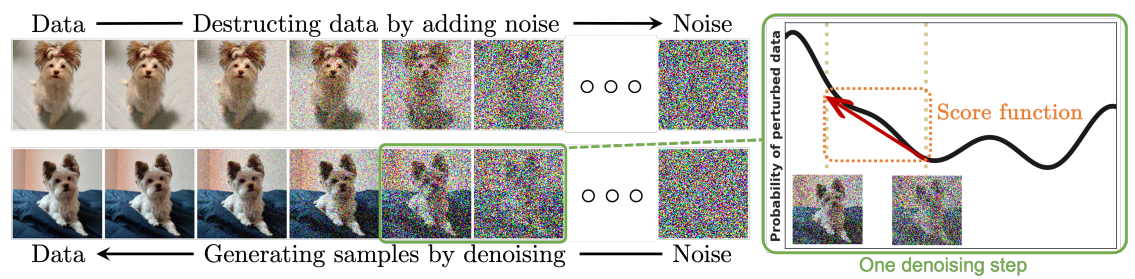
\includegraphics[width=0.5\linewidth]{imgs/Diffusion models.png}
    \caption{ Diffusion models smoothly perturb data by adding noise, then reverse this process to generate new data from noise. Each denoising step in the reverse process typically requires estimating the score function (see the illustrative figure on the right), which is a gradient pointing to the directions of data with higher likelihood and less noise. \parencite{arXiv:2209.00796}}
    \label{fig:diffusion-overview}
\end{figure}

\subsection{Forward Process}

The forward process (or the diffusion process) can be described by the following stochastic differential equation (SDE):

\begin{equation}
    dX_{t} = -\frac{1}{2}\beta(t)X_{t}dt+\sqrt{\beta(t)}dW_t \label{eq:forward-sde}
\end{equation}

Here, $X_t$ represents the data at time $t$, $\beta(t)$ is a variance schedule that governs the noise level at each step, and $dW_t$ denotes the increment of a Wiener process, reflecting the stochastic nature of the noise addition. The parameter $\beta(t)$ typically increases with $t$, indicating that the amount of noise added increases over time.

\subsection{Reverse Process}

The reverse process aims to reconstruct the original data from the noise. This is where diffusion models utilize the concept of denoising. In the reverse process, the model learns to estimate the gradients of the log probability density of the data with respect to the data itself, given the noisy data at each step. This gradient is used to perform a step-by-step denoising through the following approximate reverse SDE:

\begin{equation}
    dX_t = \left[-\frac{1}{2}\beta(t)X_t - \beta(t)\nabla_{X_t}\log p_t(X_t)\right]dt + \sqrt{\beta(t)}\mathrm{d}\bar{W}_t
    \label{eq:reverse-sde}
\end{equation}

The term $\nabla_{X_t}\log p_t(X_t)$ represents the score function that the model learns; this function guides the reverse diffusion process to effectively recover the data distribution from the noise.

\subsection{Scheduling}

The forward process in a diffusion model gradually adds noise to the original data over a series of steps. This is often done in a controlled manner according to a predefined noise schedule. The noise schedule determines the amount of noise added at each step and is typically parameterized by a variance schedule $\beta(t)$, where $t$ denotes the timestep.

The reverse process involves denoising the data. This process uses the learned parameters to gradually remove the noise from the data, aiming to revert to the original data distribution. The reverse process follows a reverse noise schedule, which ideally mirrors the forward noise schedule but in reverse order. The model learns to predict the clean data from the noisy data step-by-step, effectively learning the conditional distribution of the cleaner data given the noisier data.

The optimization of the noise schedule is a key area of research in diffusion models. The schedule needs to be carefully designed to balance the trade-offs between the model's stability, sampling speed, and quality of generated samples. Researchers often experiment with different forms of the noise schedule, such as linear, cosine, or learned schedules, each providing different benefits:

\begin{itemize}
    \item \textbf{Linear Schedules} increment noise linearly over time and are straightforward but may not always capture the nuances of more complex data distributions.
    \item \textbf{Cosine Schedules} vary noise according to a cosine function, often leading to smoother transitions in noise levels.
    \item \textbf{Learned Schedules} involve learning the noise schedule directly from the data, allowing the model to adaptively determine the best way to add and remove noise based on the specific characteristics of the data.
\end{itemize}

The experiments reported in Chapter~\ref{ch3} use the cosine schedule throughout, held fixed so that the comparison between denoising architectures is not confounded by a second varying factor. Comparing the schedules against one another would require the architecture to be held fixed instead, and is left to further work.


\chapter{Results}
\label{ch3}

\section{Experimental Configuration}

The six runs specified in Section~\ref{sec:simulation} were carried out on a single NVIDIA GeForce
RTX 4070. Every run used $T = 1000$ diffusion steps under the cosine schedule, a batch size of 128,
the Adam optimiser at a learning rate of $2 \times 10^{-4}$, thirty epochs, and random horizontal
flipping as the only augmentation. Every configuration was trained three times, under seeds 0, 1 and
2; the seed governs weight initialisation, batch order and augmentation, and within a given seed all
three architectures receive the same one. Figures below are reported as the mean over the three runs
with the sample standard deviation, and comparisons between two architectures are paired within
seed. Training used bfloat16 mixed precision with the channels-last memory format; because these
settings alter neither the model definition nor the objective, they affect the wall-clock cost of a
run but not the comparison between architectures.

Table~\ref{tab:params} records the resulting parameter budgets. The proposed network and the plain
variant are identical in size, as an identity shortcut introduces no parameters, so the comparison
between them isolates residual learning as the only variable. The reference network was narrowed
until it fell within ten per cent of the proposed network; it is in fact the smallest of the three,
which means that any advantage it shows cannot be attributed to additional capacity.

\begin{table}[htbp]
    \centering
    \caption{Parameter counts. The proposed and plain networks are identical in size by
    construction; the reference network is the smallest of the three.}
    \label{tab:params}
    \begin{tabular}{llrr}
        \toprule
        Dataset & Architecture & Parameters & Relative to ResUNet \\
        \midrule
        CIFAR-10 & ResUNet    & 2\,473\,475 & --- \\
        CIFAR-10 & plain UNet & 2\,473\,475 & $100.0\%$ \\
        CIFAR-10 & DDPM UNet  & 2\,356\,739 & $95.3\%$ \\
        \midrule
        CelebA   & ResUNet    & 2\,612\,419 & --- \\
        CelebA   & plain UNet & 2\,612\,419 & $100.0\%$ \\
        CelebA   & DDPM UNet  & 2\,356\,739 & $90.2\%$ \\
        \bottomrule
    \end{tabular}
\end{table}

\section{Training Convergence}
\label{sec:convergence}

Table~\ref{tab:loss} reports the epoch-averaged noise-prediction loss at five points during
training. Two patterns are visible, and they point in opposite directions.

\begin{table}[htbp]
    \centering
    \caption{Epoch-averaged training loss. Lower is better. The proposed network leads at the first
    epoch on both datasets and is overtaken by the fifth.}
    \label{tab:loss}
    \begin{tabular}{llccccc}
        \toprule
        & & \multicolumn{5}{c}{Epoch} \\
        \cmidrule(lr){3-7}
        Dataset & Architecture & 1 & 5 & 10 & 20 & 30 \\
        \midrule
        CIFAR-10 & ResUNet    & \textbf{0.13775} & 0.07111 & 0.06619 & 0.06249 & 0.06108 \\
        CIFAR-10 & plain UNet & 0.14633 & \textbf{0.07033} & \textbf{0.06555} & \textbf{0.06212} &
        0.06084 \\
        CIFAR-10 & DDPM UNet  & 0.18508 & 0.07135 & 0.06593 & 0.06165 & \textbf{0.05967} \\
        \midrule
        CelebA   & ResUNet    & \textbf{0.14205} & 0.04735 & 0.04110 & 0.03844 & 0.03716 \\
        CelebA   & plain UNet & 0.16413 & 0.04705 & 0.04055 & 0.03799 & 0.03679 \\
        CelebA & DDPM UNet & 0.15588 & \textbf{0.04316} & \textbf{0.03779} & \textbf{0.03573} &
        \textbf{0.03476} \\
        \bottomrule
    \end{tabular}
\end{table}

The first is an early advantage for residual learning. After a single epoch the proposed network has
the lowest loss on both datasets in every one of the three runs, ahead of the plain variant by
$5.4\%$ on average on CIFAR-10 and $11.1\%$ on CelebA. Since the two networks are identical apart
from the identity shortcut, this difference is attributable to that shortcut alone, and it is
consistent with the argument of the original ResNet work that a residual formulation is easier to
optimise than an unreferenced one.

The second pattern is that the advantage does not survive. Somewhere between the third and the sixth
epoch, depending on the seed, the plain network overtakes the proposed one on both datasets, and at
convergence it remains marginally ahead in every run, by $0.0003$ on both datasets. The direction is
consistent: the sign never changes across the six paired comparisons, and a paired test over the
three seeds gives $t(2) = 6.1$ on CIFAR-10 and $9.0$ on CelebA. The magnitude is not: $0.0003$ is
one half of one per cent of the loss. Section~\ref{sec:distribution} shows that this near-equality
on the training objective is a poor guide to the quality of the images the two networks actually
generate.

The reference network behaves differently again. It begins worst on CIFAR-10, at $0.18508$, which is
what a deeper network with more layers to coordinate would be expected to do, but it finishes with
the lowest loss on both datasets under every seed. The epoch at which it takes the lead is itself
unstable, falling anywhere between the second and the twelfth on CIFAR-10 and between the first and
the second on CelebA. The full per-epoch record is given in Appendix~\ref{sec:loss-full}.

\section{Restoration Accuracy}

The restoration diagnostics corrupt a held-out test image to a chosen timestep and measure how
completely the network recovers it in a single step. Table~\ref{tab:ssim} reports both measures over
a thousand test images at six noise levels.

\begin{table}[htbp]
    \centering
    \caption{Restoration accuracy against noise level. SSIM (higher better) above, PSNR in decibels
    (higher better) below. Differences between the proposed and plain networks are negligible
    throughout; the reference network leads at every level.}
    \label{tab:ssim}
    \begin{tabular}{lcccccccc}
        \toprule
        & \multicolumn{3}{c}{CIFAR-10} & & \multicolumn{3}{c}{CelebA} \\
        \cmidrule(lr){2-4} \cmidrule(lr){6-8}
        $t$ & ResUNet & plain & DDPM UNet & & ResUNet & plain & DDPM UNet \\
        \midrule
        \multicolumn{8}{l}{\emph{SSIM}} \\
        50  & 0.9712 & 0.9713 & \textbf{0.9713} & & 0.9708 & 0.9710 & \textbf{0.9727} \\
        100 & 0.9388 & 0.9393 & \textbf{0.9395} & & 0.9444 & 0.9451 & \textbf{0.9485} \\
        200 & 0.8701 & 0.8707 & \textbf{0.8740} & & 0.8947 & 0.8953 & \textbf{0.9027} \\
        400 & 0.7286 & 0.7281 & \textbf{0.7382} & & 0.7996 & 0.8004 & \textbf{0.8153} \\
        600 & 0.5681 & 0.5694 & \textbf{0.5826} & & 0.6891 & 0.6894 & \textbf{0.7154} \\
        800 & 0.3529 & 0.3438 & \textbf{0.3642} & & 0.5117 & 0.5023 & \textbf{0.5510} \\
        \emph{Mean} & 0.7383 & 0.7371 & \textbf{0.7450} & & 0.8017 & 0.8006 & \textbf{0.8176} \\
        \midrule
        \multicolumn{8}{l}{\emph{PSNR} (dB)} \\
        50  & 33.50 & 33.52 & \textbf{33.54} & & 35.51 & 35.54 & \textbf{35.77} \\
        100 & 29.89 & 29.91 & \textbf{29.95} & & 32.20 & 32.24 & \textbf{32.49} \\
        200 & 26.21 & 26.23 & \textbf{26.34} & & 28.80 & 28.83 & \textbf{29.10} \\
        400 & 22.35 & 22.37 & \textbf{22.52} & & 25.07 & 25.10 & \textbf{25.40} \\
        600 & 19.61 & 19.61 & \textbf{19.80} & & 22.23 & 22.25 & \textbf{22.61} \\
        800 & 16.63 & 16.50 & \textbf{16.87} & & 18.82 & 18.74 & \textbf{19.18} \\
        \emph{Mean} & 24.70 & 24.69 & \textbf{24.84} & & 27.10 & 27.12 & \textbf{27.43} \\
        \bottomrule
    \end{tabular}
\end{table}

Three observations follow. The first is that at $t = 50$ the three networks are indistinguishable to
four decimal places on SSIM and to within $0.04$\,dB on PSNR. An image at that noise level is barely
corrupted, and almost any denoiser recovers it; the measurement discriminates only as the corruption
grows.

The second is that the proposed and plain networks cannot be separated. Their mean SSIM differs by
$0.0012$ on CIFAR-10 and $0.0011$ on CelebA, and their mean PSNR by $0.01$\,dB and $0.02$\,dB.
Repeating the whole procedure under three seeds puts those figures in context. The seed-to-seed
standard deviation of mean SSIM is $0.0013$ for the proposed network and $0.0030$ for the plain one
on CIFAR-10, which is of the same order as the $0.0031$ that separates them. The paired differences
do favour the proposed network consistently, at $t(2) = 2.0$ on CIFAR-10 and $2.4$ on CelebA, but
they run in the opposite direction to the training loss, and PSNR changes sign between seeds
altogether. The restoration measures are individually stable and jointly inconclusive: they can be
trusted to a thousandth, and at that resolution they do not agree on which network is better.

The third is that the reference network leads at every noise level on both datasets and on both
measures, and its margin grows with $t$. Its advantage is consistently larger on CelebA than on
CIFAR-10, which is the pattern the higher resolution was introduced to expose.

\section{Distribution-Level Quality}
\label{sec:distribution}

The measures reported so far compare the networks as denoisers. Table~\ref{tab:fid} compares them as
generators, using 2048 samples drawn from each model through the complete thousand-step reverse
process.

\begin{table}[htbp]
    \centering
    \caption{Fr\'echet Inception Distance from 2048 samples per model, for each of the three
    seeds, with the mean and sample standard deviation. Lower is better.}
    \label{tab:fid}
    \begin{tabular}{llrrrr}
        \toprule
        Dataset & Architecture & Seed 0 & Seed 1 & Seed 2 & Mean $\pm$ SD \\
        \midrule
        CIFAR-10 & ResUNet    & $94.93$ & $128.23$ & $89.03$ & $104.07 \pm 21.13$ \\
        CIFAR-10 & plain UNet & $84.29$ & $145.12$ & $93.15$ & $107.52 \pm 32.86$ \\
        CIFAR-10 & DDPM UNet  & $68.09$ & $68.66$ & $81.88$ & $\mathbf{72.88 \pm 7.80}$ \\
        \midrule
        CelebA   & ResUNet    & $76.06$ & $109.79$ & $63.40$ & $83.08 \pm 23.98$ \\
        CelebA   & plain UNet & $135.18$ & $131.47$ & $172.53$ & $146.39 \pm 22.71$ \\
        CelebA   & DDPM UNet  & $76.93$ & $73.91$ & $93.87$ & $\mathbf{81.57 \pm 10.76}$ \\
        \bottomrule
    \end{tabular}
\end{table}

This table carries the most important result of the project, and the three seeds are what make it
readable. The seed-to-seed standard deviation of FID runs from $7.8$ to $32.9$, an order of
magnitude larger than the variation of any restoration measure, so a comparison drawn from a single
run of this length cannot be relied upon. Two of the three comparisons available here dissolve under
repetition; one does not.

On CIFAR-10 the proposed and plain networks cannot be separated. Their means are $104.07$ and
$107.52$, the paired difference is $-3.46$ against a standard deviation of $13.78$, and the sign
changes between seeds: the proposed network is worse by $10.64$ under seed 0, better by $16.89$
under seed 1 and better by $4.12$ under seed 2. A paired test gives $t(2) = -0.43$. At two
resolution stages the identity shortcut makes no difference to generative quality that this
experiment can detect.

On CelebA it does. The proposed network is ahead in all three runs, by $59.12$, $21.68$ and
$109.13$, for a mean advantage of $63.31$ FID. That gap is larger than the seed-to-seed standard
deviation of either network, $23.98$ and $22.71$, and the direction never changes. The evidence is
not conclusive at this sample size, a paired test giving $t(2) = -2.50$, which does not reach
significance with two degrees of freedom, but a consistent advantage of that size across three
independent runs is not readily explained as noise.

The reference architecture leads on CIFAR-10 by $31.19$ FID over the proposed network, in every
seed, and is also the most stable of the three, with a standard deviation of $7.80$ against $21.13$
and $32.86$. On CelebA it is matched: the mean difference to the proposed network is $1.51$ FID with
a standard deviation of $33.24$, and the sign is mixed. Its Inception Score on CIFAR-10, $5.655$
against $4.711$ and $4.625$, agrees with its FID lead.

Read together with the previous section, the two sets of measurements are in tension. The
restoration measures are stable to a thousandth but cannot separate the proposed and plain networks,
and where they do lean they contradict one another. FID separates them decisively on CelebA but
varies by tens of points between seeds. The measurement that is reliable is uninformative, and the
measurement that is informative is noisy. The reason is the same in both cases: the training
objective and the restoration diagnostics both average the noise-prediction error over timesteps,
whereas generation composes a thousand such predictions in sequence, and errors that are small on
average but systematic at particular timesteps compound through that composition. A network can be
an excellent denoiser and a poor generator, and only a distribution-level measure sees it.

The difference between the two datasets invites an explanation in terms of depth. At $32 \times 32$
the proposed network has two resolution stages and the shortcut changes nothing; at $64 \times 64$
it has three and the shortcut is worth sixty FID points. Residual connections exist to make deeper
networks optimisable, so a benefit that appears only in the deeper configuration is what the
original argument would predict. The present experiment cannot establish this, because depth and
resolution vary together; separating them would require the two-stage and three-stage networks to be
trained on the same images.

\section{Memorisation}

Because the CelebA samples are recognisable faces, it is necessary to establish that the models are
generating rather than reproducing. Table~\ref{tab:nn} reports the mean distance from each generated
sample to its nearest training image, against two controls.

\begin{table}[htbp]
    \centering
    \caption{Mean pixel-space $L_2$ distance to the nearest training image. A generated sample that
    is no closer than a blurred real image gives no evidence of reproduction.}
    \label{tab:nn}
    \begin{tabular}{lrrr|rrr}
        \toprule
        & \multicolumn{3}{c|}{CIFAR-10} & \multicolumn{3}{c}{CelebA} \\
        & ResUNet & plain & DDPM & ResUNet & plain & DDPM \\
        \midrule
        Generated            & 18.00 & 16.93 & 17.06 & 43.94 & 47.02 & 43.56 \\
        \midrule
        Real held-out images & \multicolumn{3}{c|}{18.68} & \multicolumn{3}{c}{38.41} \\
        Blurred held-out     & \multicolumn{3}{c|}{16.09} & \multicolumn{3}{c}{35.97} \\
        \bottomrule
    \end{tabular}
\end{table}

On CelebA every model produces samples that are \emph{further} from the training set than genuine
unseen photographs are, by between thirteen and twenty-two per cent, which settles the question
directly.

CIFAR-10 requires the second control. The generated samples sit slightly closer to the training set
than real held-out images do, at between $0.91$ and $0.96$ of the reference distance, and taken
alone that could be read as mild reproduction. Blurring a real held-out image with a $3 \times 3$
mean filter, however, reduces its distance to $16.09$, or $0.86$ of the reference. Smoothing an
image moves it towards the mean of the data and therefore towards everything in it. All three models
remain further away than that purely smoothing-induced floor, so the shortfall is explained by the
softness of samples from an undertrained model rather than by copying.

Figure~\ref{fig:memorisation} shows the eight closest generated and training pairs for the proposed
network on CelebA. The nearest training image is a different person in every case.

\begin{figure}[htbp]
    \centering
    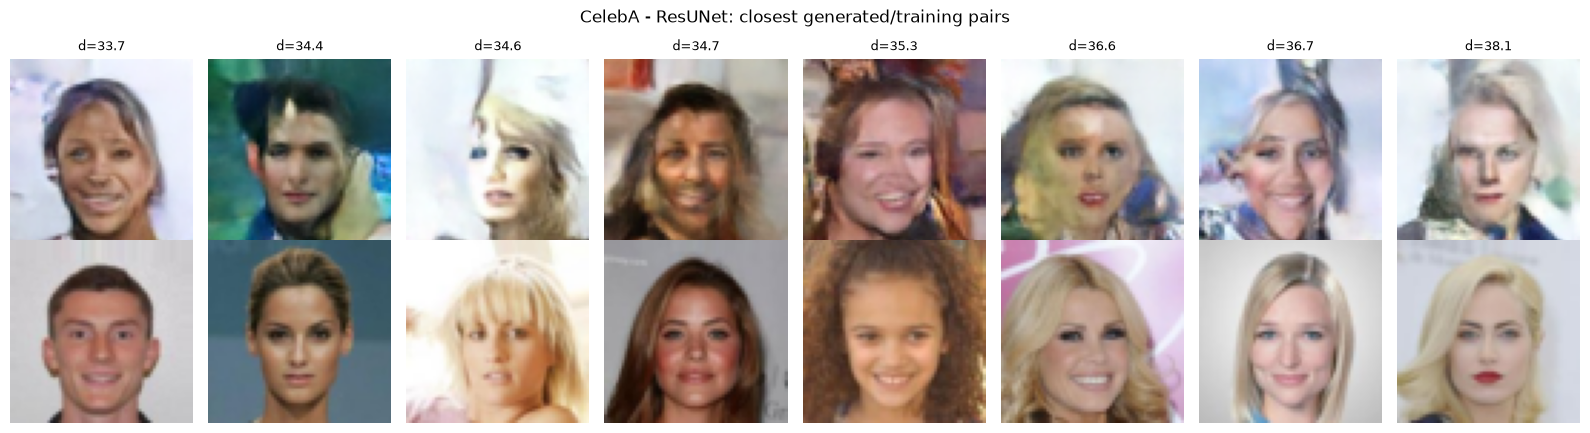
\includegraphics[width=\linewidth]{memo_celeba_resunet.png}
    \caption{The eight CelebA samples closest to the training set (top) with their nearest training
    image (bottom), for the proposed network. No pair depicts the same person.}
    \label{fig:memorisation}
\end{figure}

\section{Computational Cost}

Table~\ref{tab:cost} records the steady-state time for one training epoch. The proposed and plain
networks are within two per cent of one another on both datasets, confirming in practice what the
parameter counts assert in principle: removing an identity shortcut changes neither the parameter
count nor the arithmetic performed.

\begin{table}[htbp]
    \centering
    \caption{Steady-state training time per epoch. The first epoch of each dataset absorbs
    convolution autotuning and is excluded.}
    \label{tab:cost}
    \begin{tabular}{lccc}
        \toprule
        Dataset & ResUNet & plain UNet & DDPM UNet \\
        \midrule
        CIFAR-10 ($32 \times 32$) & $16.0$\,s & $15.8$\,s & $38.5$\,s \\
        CelebA ($64 \times 64$)   & $32.0$\,s & $31.4$\,s & $68.3$\,s \\
        \bottomrule
    \end{tabular}
\end{table}

The reference network costs $2.4$ times as much per epoch on CIFAR-10 and $2.2$ times as much on
CelebA, despite having fewer parameters than either competitor. The cost is incurred by depth and by
attention rather than by weight count. Its advantage on CIFAR-10 is decisive and justifies the
additional cost; on CelebA it is matched by the proposed network at less than half the training
cost.

\section{Generated Samples}

\subsection{A Note on the Reverse Process}
\label{sec:reverse-note}

The first attempt at unconditional sampling produced saturated noise from every model. The cause was
not the models but the implementation of the reverse step. Writing the posterior mean directly as
$\left(x_t - \frac{\beta_t}{\sqrt{1-\bar\alpha_t}}\varepsilon_\theta\right)/\sqrt{\alpha_t}$ is
algebraically correct only while the implied estimate of $x_0$ remains inside the data range. The
factor $1/\sqrt{\alpha_t}$ reaches $31.6$ at $t = 999$ under the clipped cosine schedule, so any
error in $\varepsilon_\theta$ is amplified by that factor and accumulates over the thousand steps of
the reverse process. Tracing the sample statistics confirmed the effect: the standard deviation of
$x$ grew from $1.0$ at the start of the trajectory to approximately $16$ by its end, and over $95\%$
of pixels finished outside the valid range. The same divergence occurred in single precision, which
excludes reduced precision as the cause.

The remedy is the one used in the reference implementation: recover $x_0$ explicitly, clip it to
$[-1, 1]$, and rebuild the posterior mean from the clipped estimate. With this correction the
terminal standard deviation falls to between $0.48$ and $0.64$ across the six models, matching the
scale of the training data, and no pixel leaves the valid range. All samples reported here use the
corrected procedure. The episode illustrates a property of the reverse process that the forward
derivation does not make obvious: the algebraic form of the posterior mean is stable only for a
network that is already accurate, and the clipping step is what makes sampling robust to a network
that is not.

\subsection{Samples}

Figure~\ref{fig:samples-cifar} and Figure~\ref{fig:samples-celeba} show sixty-four samples drawn
from each model. Every model was given the same initial noise, so differences between the panels are
attributable to the denoising network.

\begin{figure}[htbp]
    \centering
    \begin{minipage}{0.31\linewidth}
        \centering
        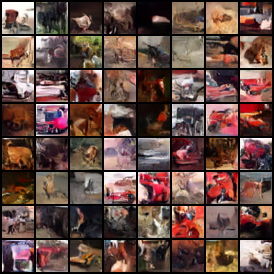
\includegraphics[width=\linewidth]{samples_CIFAR-10_resunet.png}\\[2mm]
        {\small ResUNet}
    \end{minipage}\hfill
    \begin{minipage}{0.31\linewidth}
        \centering
        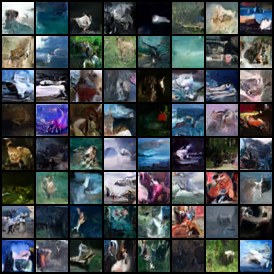
\includegraphics[width=\linewidth]{samples_CIFAR-10_plain.png}\\[2mm]
        {\small plain UNet}
    \end{minipage}\hfill
    \begin{minipage}{0.31\linewidth}
        \centering
        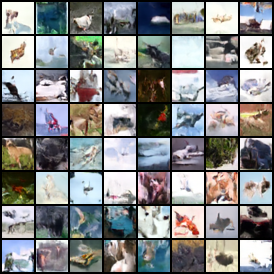
\includegraphics[width=\linewidth]{samples_CIFAR-10_ddpm_unet.png}\\[2mm]
        {\small DDPM UNet}
    \end{minipage}
    \caption{Unconditional CIFAR-10 samples after thirty epochs, all three models starting from
    identical noise.}
    \label{fig:samples-cifar}
\end{figure}

\begin{figure}[htbp]
    \centering
    \begin{minipage}{0.31\linewidth}
        \centering
        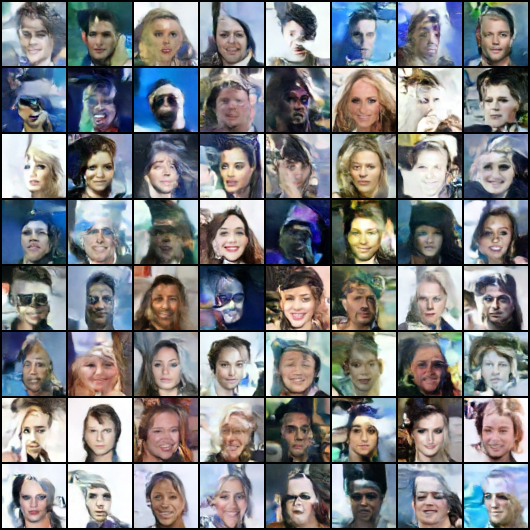
\includegraphics[width=\linewidth]{samples_CelebA_resunet.png}\\[2mm]
        {\small ResUNet}
    \end{minipage}\hfill
    \begin{minipage}{0.31\linewidth}
        \centering
        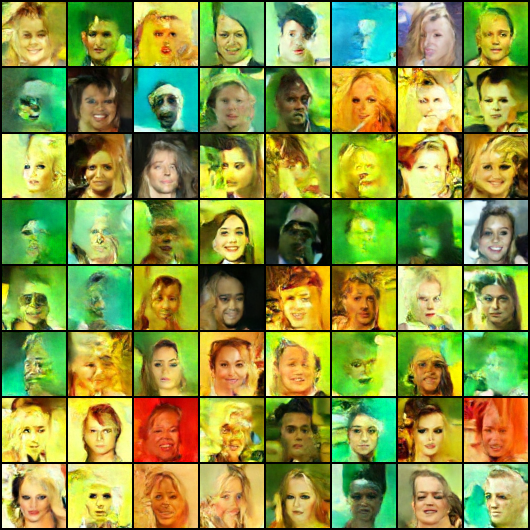
\includegraphics[width=\linewidth]{samples_CelebA_plain.png}\\[2mm]
        {\small plain UNet}
    \end{minipage}\hfill
    \begin{minipage}{0.31\linewidth}
        \centering
        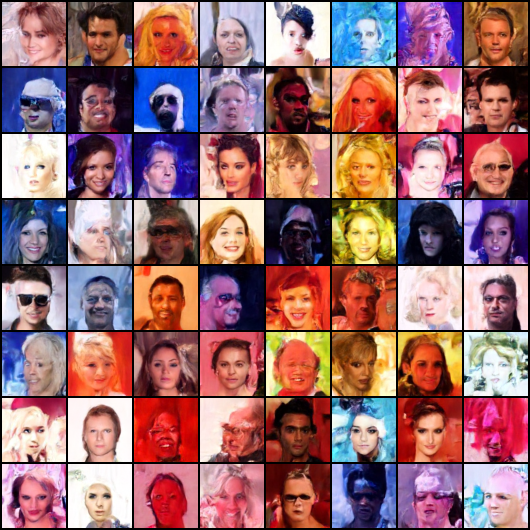
\includegraphics[width=\linewidth]{samples_CelebA_ddpm_unet.png}\\[2mm]
        {\small DDPM UNet}
    \end{minipage}
    \caption{Unconditional CelebA samples at $64 \times 64$ after thirty epochs, all three models
    starting from identical noise.}
    \label{fig:samples-celeba}
\end{figure}

On CIFAR-10 all three models produce coherent local texture and plausible figure-ground separation,
and some samples suggest recognisable categories such as animals or vehicles, but none is
identifiable with confidence. This is the expected outcome for networks of two and a half million
parameters trained for eleven thousand optimisation steps; the published CIFAR-10 configuration is
roughly fourteen times larger and is trained for nearly seventy times as many steps.

The CelebA panels are where the FID result becomes visible. All three models generate face-like
images with correct global arrangement, but the plain network's faces are noticeably less coherent,
with more frequent failures of facial structure, which is consistent with its FID of $135.18$
against $76.06$ and $76.93$ for the other two. The proposed and reference networks are difficult to
separate by eye, as their almost identical scores would suggest. Colour saturation is exaggerated in
all three, a known consequence of clipping the estimate of $x_0$ at every step of an undertrained
reverse process.

\subsection{Why the Samples Are Indistinct}
\label{sec:indistinct}

The samples above are recognisable in kind but not in particular, and it is worth separating the two
reasons for that, because only one of them is a property of the method.

The first is simply the scale of the experiment. Table~\ref{tab:budget} sets the configuration used
here beside the one published with the original DDPM \parencite{arXiv:2006.11239}. The networks
trained for this work are roughly fourteen times smaller and receive sixty-eight times fewer
optimisation steps, which places the total training computation about three orders of magnitude
below the reference. The resulting Fr\'echet Inception Distance is about twenty times worse. Nothing
in that comparison is surprising, and it is the reason Section~\ref{sec:distribution} treats only
the relative ordering of the three networks as meaningful.

\begin{table}[htbp]
    \centering
    \caption{Training budget compared with the published CIFAR-10 configuration. The difference in
    computation is approximately three orders of magnitude.}
    \label{tab:budget}
    \begin{tabular}{lrrr}
        \toprule
        & This work & Ho et al. & Ratio \\
        \midrule
        Parameters & 2.47\,M & 35.7\,M & $14\times$ \\
        Optimisation steps & 11\,700 & 800\,000 & $68\times$ \\
        Relative computation & $1$ & $\approx 10^{3}$ & $\approx 10^{3}$ \\
        CIFAR-10 FID & $68.09$ & $\approx 3.17$ & $21\times$ \\
        \bottomrule
    \end{tabular}
\end{table}

The second reason explains why the failure takes the particular form of indistinctness rather than,
say, visible artefacts. The training objective is a squared error, and when a network is uncertain
the prediction that minimises squared error is the average of the outcomes it considers possible.
Averaging over several plausible completions of a region produces a smooth one. This is the same
mechanism that gives Variational Autoencoders their characteristic softness, discussed in
Section~\ref{sec:vae}, and it is not specific to either architecture tested here.

What distinguishes a diffusion model is that it does not have to commit to a whole image at once.
Dividing the task into a thousand steps keeps the uncertainty at each step small, and the noise
added back at every step, in the term $\sigma_t z$ of the reverse process, pushes the trajectory
towards one specific outcome instead of the average of many. Both mitigations depend on each step
being accurate. An undertrained network makes a small error at every one of the thousand steps, the
averaging reasserts itself, and the softness returns. The indistinctness observed here is therefore
a symptom of the training budget rather than of the formulation, and the remedies set out in the
Conclusions are addressed to that budget.

Figure~\ref{fig:trajectory} shows the reverse trajectory of the proposed network on both datasets,
sampled every twenty steps. Structure emerges late: the first two thirds of the trajectory refine
what remains essentially noise, and the recognisable image forms over the final few hundred steps.

\begin{figure}[htbp]
    \centering
    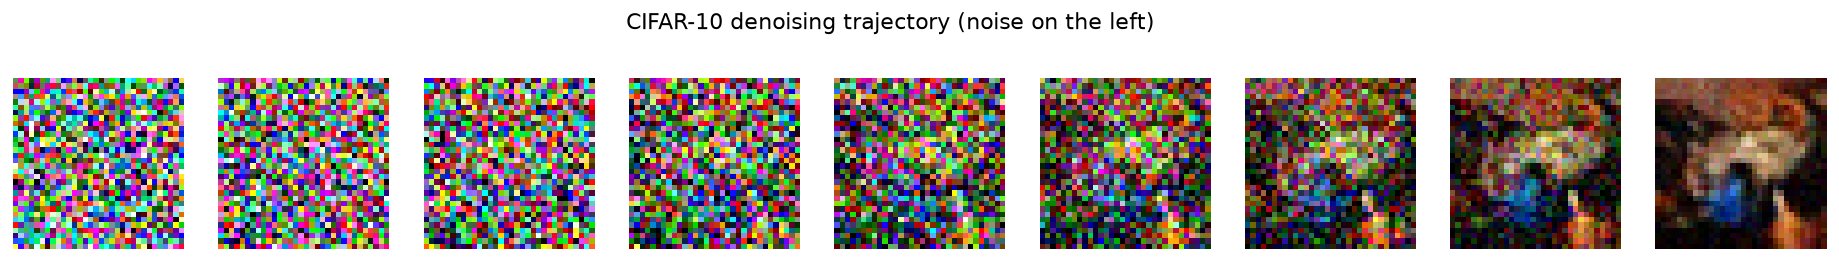
\includegraphics[width=\linewidth]{denoise_traj_cifar10.png}\\[3mm]
    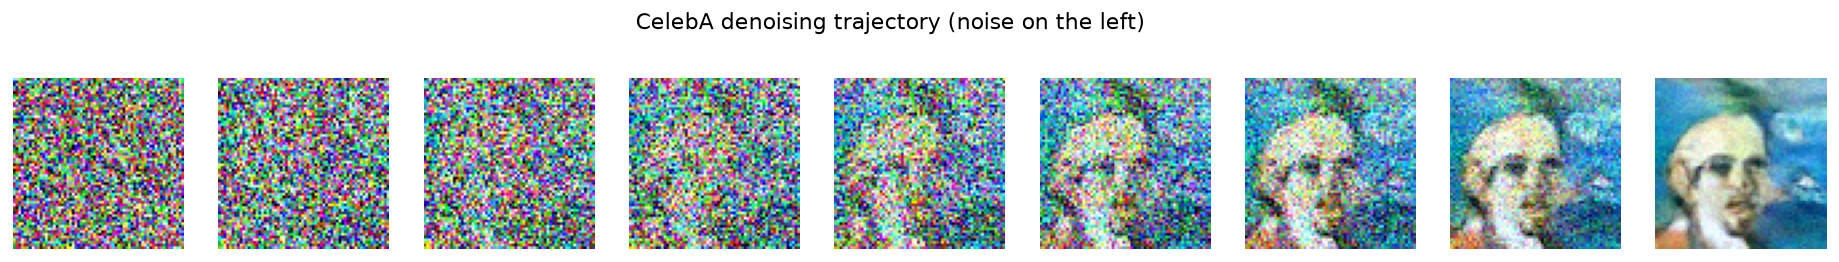
\includegraphics[width=\linewidth]{denoise_traj_celeba.png}
    \caption{Reverse trajectories of the proposed network on CIFAR-10 (top) and CelebA (bottom),
    with pure noise on the left and the final sample on the right.}
    \label{fig:trajectory}
\end{figure}

\section{Summary}

Figure~\ref{fig:comparison} collects the training curves and the restoration measurements. Four
findings follow from the experiment.

\begin{figure}[htbp]
    \centering
    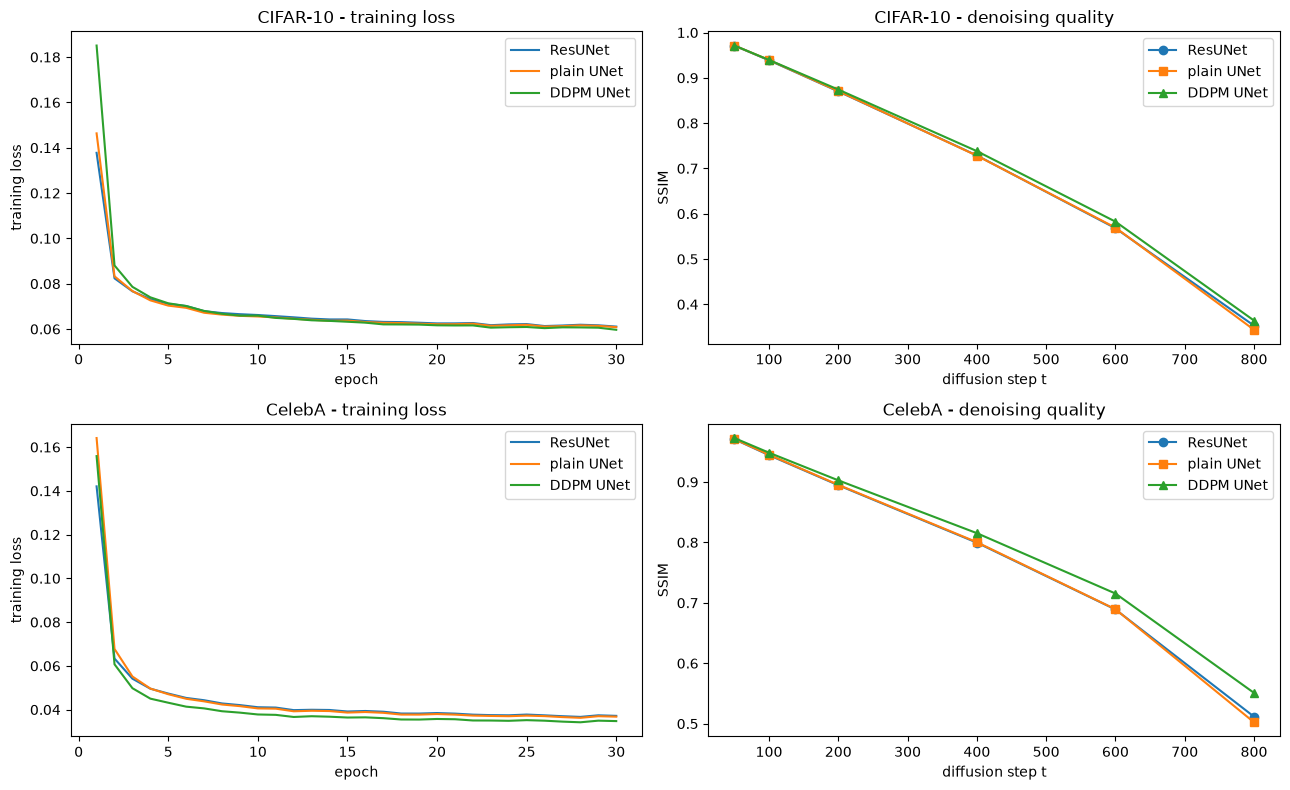
\includegraphics[width=\linewidth]{results_comparison.png}
    \caption{Training loss (left) and denoising accuracy against noise level (right) for CIFAR-10
    (top) and CelebA (bottom).}
    \label{fig:comparison}
\end{figure}

\begin{itemize}
    \item \textbf{Residual shortcuts accelerate early optimisation.} The proposed network reaches a
    lower loss than its shortcut-free twin after a single epoch in all six paired runs, by $5.4\%$
    on average on CIFAR-10 and $11.1\%$ on CelebA. As the two networks are otherwise identical, the
    shortcut is the only possible cause.

    \item \textbf{Restoration measures cannot separate the two networks.} Their final training loss,
    mean SSIM and mean PSNR agree to within half of one per cent, and the two that lean at all lean
    in opposite directions: the loss favours the plain network in every run, SSIM favours the
    proposed one, and PSNR changes sign between seeds.

    \item \textbf{Generative quality separates them on the deeper configuration only.} At
    $64 \times 64$, where the proposed network has three resolution stages, it leads in all three
    seeds by a mean of $63.31$ FID. At $32 \times 32$, with two stages, the sign changes between
    seeds and the paired difference is $-3.46 \pm 13.78$. Networks that denoise identically well do
    not generate equally well, and no restoration measure predicted it.

    \item \textbf{The reference architecture remains the strongest overall.} It leads every
    restoration measure on both datasets and CIFAR-10 FID by $31.19$ in every seed, using fewer
    parameters than either competitor, at roughly $2.3$ times the training cost. It is also the most
    stable, with an FID standard deviation of $7.80$ against $21.13$ and $32.86$. Only on CelebA FID
    is it matched, by the proposed network at less than half the cost.
\end{itemize}

The hypothesis stated in Chapter~\ref{ch1} therefore receives partial and conditional support. The
combination of residual learning with a UNet backbone does not improve the quality of generated
images in general; at two resolution stages it makes no difference this experiment can detect. At
three stages, where the network is deep enough for the optimisation difficulty that residual
learning was invented to address, the proposed network leads in every seed by a margin larger than
the seed-to-seed variation, and that advantage is invisible to every measure except the
distribution-level one. Three seeds are not enough to place a confidence interval on the claim, but
they are enough to show that the two-stage result of a single run was noise and the three-stage
result was not.

\chapter{Extension}
\label{ch4}

Section~\ref{sec:indistinct} attributed the indistinctness of the samples in Chapter~\ref{ch3} to
two causes: a training budget roughly three orders of magnitude below the published configuration,
and the tendency of a squared-error objective to regress towards the mean wherever the network is
uncertain. The Conclusions proposed remedies for both. This chapter carries them out.

The question changes accordingly. Chapter~\ref{ch3} asked which of three denoising networks
generates the best images when all are trained identically; this chapter holds the proposed ResUNet
and the diffusion framework fixed and asks how much of the gap to the published result can be closed
by changing only how the network is trained and sampled. The changes are applied one at a time as a
cumulative ladder, so that the contribution of each can be read from the difference between adjacent
rungs.

% 결과는 주말 72시간 실행(DissertationExtension.ipynb, PRESET = "full")이 끝난 뒤
% model/extension/extension_study.json 에서 4.7절 표로 옮긴다
Sections~\ref{sec:ext-motivation} to~\ref{sec:ext-budget} set out the design, the reasoning behind
every change and the computational budget. Section~\ref{sec:ext-results} states in advance how the
results are to be read and reports them once the runs are complete.

\section{Motivation}
\label{sec:ext-motivation}

The two causes identified in Chapter~\ref{ch3} call for different remedies, and it is worth stating
each precisely.

The first is scale. The networks of Chapter~\ref{ch3} have 2.47 million parameters and were trained
for 11\,700 optimisation steps, against 35.7 million parameters and 800\,000 steps for the CIFAR-10
configuration of Ho et al.\ \parencite{arXiv:2006.11239} (Table~\ref{tab:budget}). Of the two
ratios, the one in steps is the larger by a factor of five, and so is the first target here.

The second is a property of the objective. The network is trained to minimise
\begin{equation}
    \mathcal{L}_{\text{simple}} = \mathbb{E}_{t,\,x_0,\,\varepsilon}
    \left[\left\lVert \varepsilon - \varepsilon_\theta(x_t, t) \right\rVert^2\right],
    \qquad x_t = \sqrt{\bar\alpha_t}\,x_0 + \sqrt{1-\bar\alpha_t}\,\varepsilon,
    \label{eq:ext-simple-loss}
\end{equation}
and the function that minimises a squared error is the conditional expectation of its target,
\begin{equation}
    \varepsilon_\theta^{*}(x_t, t) = \mathbb{E}\left[\varepsilon \mid x_t\right]
    \quad\Longrightarrow\quad
    \hat{x}_0 = \frac{x_t - \sqrt{1-\bar\alpha_t}\,\varepsilon_\theta^{*}(x_t, t)}{\sqrt{\bar\alpha_t}}
    = \mathbb{E}\left[x_0 \mid x_t\right].
    \label{eq:ext-cond-mean}
\end{equation}
Where several clean images are consistent with a noisy one, the ideal network therefore predicts
their average, and the average of several plausible images is smoother than any of them. The
reverse process counteracts this by committing to one outcome a little at a time, as argued in
Section~\ref{sec:indistinct}, but only if each of its thousand predictions is accurate. Anything
that reduces the error of an individual prediction, including noise in the weights themselves,
therefore also addresses the second cause.

\section{Experimental Design}
\label{sec:ext-design}

\subsection{What Is Held Fixed}

Everything that defines the generative model is unchanged from Chapter~\ref{ch3}: $T = 1000$
diffusion steps under the cosine schedule \parencite{arXiv:2102.09672}, the $\varepsilon$-prediction
objective, the ancestral sampler with the estimate of $x_0$ clipped at every step
(Section~\ref{sec:reverse-note}), the ResUNet family of Section~\ref{sec:simulation}, a batch size
of 128, the Adam optimiser \parencite{arXiv:1412.6980} at a learning rate of $2 \times 10^{-4}$,
random horizontal flipping, seed~0, and a Fr\'echet Inception Distance computed from 2048 samples.
Every sample in every rung is drawn from the same initial noise.

\subsection{The Ladder}

Table~\ref{tab:ladder} lists the seven rungs. Each inherits every setting of the one above it and
changes one thing, so the difference in FID between adjacent rungs,
\begin{equation}
    \Delta\mathrm{FID}_i = \mathrm{FID}(E_i) - \mathrm{FID}(E_{i-1}),
    \label{eq:ext-delta}
\end{equation}
is attributable to that change. Two qualifications apply. Three rungs (E2, E5 and E6) change more
than one setting at once, for reasons given below, and their contributions cannot be divided further.
And because the ladder is cumulative, each contribution is measured in the presence of all the
changes that precede it; applied in a different order, a change could contribute a different amount.

\begin{table}[htbp]
    \centering
    \caption{The cumulative ladder. Each rung adds the change in its row to all of those above it.
    Widths are listed for CIFAR-10; the corresponding CelebA widths are $(32, 64, 128)$ and
    $(96, 192, 256)$.}
    \label{tab:ladder}
    \small
    \begin{tabular}{llrlc}
        \toprule
        Rung & Change added & Epochs & Widths & Blocks per stage \\
        \midrule
        E0 & none (Chapter~\ref{ch3}, seed 0)            & 30  & $(64, 128)$ & 1 \\
        E1 & moving average of the weights              & 30  & $(64, 128)$ & 1 \\
        E2 & warm-up, gradient clipping, dropout        & 30  & $(64, 128)$ & 1 \\
        E3 & min-SNR loss weighting, $\gamma = 5$         & 30  & $(64, 128)$ & 1 \\
        E4 & five times the training                      & 150 & $(64, 128)$ & 1 \\
        E5 & increased capacity                           & 150 & $(128, 256, 256)$ & 2 \\
        E6 & long training, EMA decay 0.9999              & 2000\textsuperscript{a} &
        $(128, 256, 256)$ & 2 \\
        \bottomrule
        \multicolumn{5}{l}{\footnotesize \textsuperscript{a} 700 on CelebA; see
        Section~\ref{sec:ext-long}.}
    \end{tabular}
\end{table}

The complete ladder is run on CIFAR-10, which is where the contribution of each change is isolated.
On CelebA only E0, E5 and E6 are run. The purpose there is to establish whether the overall effect
carries over to a second dataset at twice the resolution, and the difference between the first rung
and the last is sufficient for that.

\subsection{Validation of the Starting Point}

E0 repeats the seed-0 ResUNet run of Chapter~\ref{ch3} exactly, and serves as a check on the new
pipeline: if it did not reproduce the earlier result, no other row could be trusted. The criterion
adopted is agreement within one seed-to-seed standard deviation of that result, which
Table~\ref{tab:fid} puts at $21.13$ for this network on CIFAR-10. A preliminary evaluation of the E0
checkpoint gives an FID of $89.57$ against the $94.93$ of Chapter~\ref{ch3}, a difference of $5.36$,
well inside that criterion.

\section{Rationale for Each Change}
\label{sec:ext-rationale}

\subsection{Exponential Moving Average of the Weights (E1)}
\label{sec:ext-ema}

Stochastic gradient descent at a constant learning rate does not settle at a minimum; it fluctuates
around one, with an amplitude governed by the learning rate and the variance of the gradient. The
last iterate is one draw from that fluctuation. Polyak and Juditsky showed that the average of the
iterates is a better estimate of the minimum than any single one of them, and converges at the
optimal rate \parencite{polyak1992averaging}. Diffusion models apply the same idea as an exponential
moving average,
\begin{equation}
    \bar\theta_k = d_k\,\bar\theta_{k-1} + (1 - d_k)\,\theta_k,
    \qquad d_k = \min\!\left(d,\; \frac{1 + k}{10 + k}\right),
    \label{eq:ext-ema}
\end{equation}
where $\theta_k$ are the weights after step $k$ and $\bar\theta_k$ the averaged copy. Training
continues on $\theta_k$; only sampling uses $\bar\theta_k$. The practice is standard in the
diffusion literature: Ho et al.\ sample from an average with $d = 0.9999$
\parencite{arXiv:2006.11239}, and Song and Ermon identify it as one of the techniques on which the
stability of score-based models depends \parencite{arXiv:2006.09011}.

For a constant decay the average places weight $(1-d)\,d^{\,k-j}$ on the iterate $j$ steps in the
past, so it effectively averages over the last $1/(1-d)$ steps. The warm-up in
Equation~\eqref{eq:ext-ema} exists because a constant decay misbehaves in a short run. With
$d = 0.9999$ and no warm-up, a quantity $d^{\,k}$ of the average still belongs to the random
initialisation after $k$ steps, which is $31\%$ at the end of a 30-epoch run of 11\,700 steps. Under
the warm-up the effective window grows as $(10 + k)/9$, so the average always covers roughly the most
recent ninth of training, until the window reaches the cap $1/(1-d)$ at step $(10d - 1)/(1 - d)$.
Figure~\ref{fig:ext-ema-window} shows the resulting window against the length of each rung.

\begin{figure}[htbp]
    \centering
    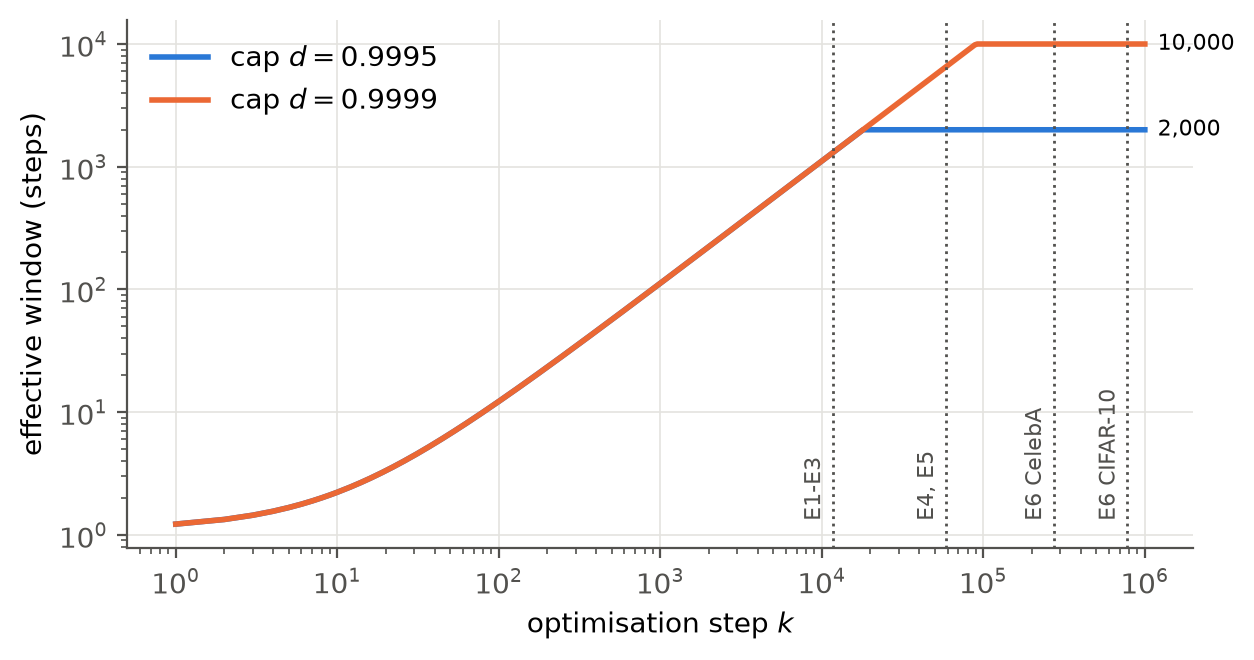
\includegraphics[width=0.8\linewidth]{ext_ema_window.png}
    \caption{Effective averaging window $1/(1 - d_k)$ of the moving average in
    Equation~\eqref{eq:ext-ema}. The two caps coincide throughout the warm-up, which ends at step
    17\,990 for $d = 0.9995$ and at step 89\,990 for $d = 0.9999$. Dotted lines mark the length of
    each rung. Drawn from Equation~\eqref{eq:ext-ema}.}
    \label{fig:ext-ema-window}
\end{figure}

Two consequences follow. The first is that the thirty-epoch rungs E1 to E3 end at step 11\,700,
before either cap is reached, so their average is determined by the warm-up alone and the choice of
cap has no effect on them. The second is that the cap matters only for the long rungs, and there it
sets a trade-off between variance and lag. A longer window averages out more of the fluctuation but
also trails further behind weights that are still improving. E4 and E5 use $d = 0.9995$, whose window
of 2000 steps is about five epochs and $3.4\%$ of the run. E6 uses $d = 0.9999$, the value of Ho et
al., whose window of 10\,000 steps is $1.3\%$ of its 780\,000; late in a run of that length the
weights drift slowly enough that the longer average costs little in lag. The change of cap is part
of E6 rather than a rung of its own for this reason, since it is a consequence of the length of
training rather than an independent choice.

\subsection{Learning-Rate Warm-Up, Gradient Clipping and Dropout (E2)}
\label{sec:ext-stabilisers}

The three changes in E2 share a purpose. Each makes training more robust without altering what is
being learned, each is used in the reference implementation of Ho et al., and each is expected to
have a small effect individually at thirty epochs. Giving each a rung of its own would have added two
thirty-epoch runs to measure differences that a single seed could not resolve.

\paragraph{Warm-up.} Adam scales each step by a running estimate of the second moment of the
gradient,
\begin{equation}
    \theta_{k+1} = \theta_k - \eta_k\,\frac{\hat m_k}{\sqrt{\hat v_k} + \epsilon},
    \label{eq:ext-adam}
\end{equation}
where $\hat m_k$ and $\hat v_k$ are the bias-corrected first and second moment estimates
\parencite{arXiv:1412.6980}. In the first steps $\hat v_k$ is estimated from very few gradients, and
Liu et al.\ show that the variance of the resulting adaptive learning rate is then large enough to
drive training towards poor regions of the loss surface \parencite{arXiv:1908.03265}. A linear warm-up,
\begin{equation}
    \eta_k = \eta\,\min\!\left(1,\; \frac{k+1}{K}\right),
    \label{eq:ext-warmup}
\end{equation}
keeps the step small until the estimate has settled. The same device is used to stabilise training
at large batch sizes \parencite{arXiv:1706.02677}. The reference implementation uses $K = 5000$; a
value of $K = 2000$ is used here because the thirty-epoch rungs last only 11\,700 steps, and 5000
would spend $43\%$ of them warming up against $17\%$ for 2000.

\paragraph{Gradient clipping.} The training loss mixes timesteps of very different difficulty, and
an occasional batch produces a gradient far larger than typical. Rescaling the gradient whenever its
norm exceeds a threshold $c$,
\begin{equation}
    g \leftarrow g \cdot \min\!\left(1,\; \frac{c}{\lVert g \rVert_2}\right),
    \label{eq:ext-clip}
\end{equation}
bounds the size of the step while preserving its direction. The technique was introduced to control
exploding gradients in recurrent networks \parencite{arXiv:1211.5063}; $c = 1$ is the value of the
reference implementation, and the norm is taken over all parameters together.

\paragraph{Dropout.} Rungs E4 to E6 pass over the same fifty thousand images between 150 and 2000
times, and a network trained that long can begin to fit its training set rather than the
distribution behind it. Dropout counters this by zeroing each activation independently with
probability $p$ during training and rescaling the survivors,
\begin{equation}
    \tilde h = \frac{m \odot h}{1 - p}, \qquad m_i \sim \mathrm{Bernoulli}(1 - p),
    \label{eq:ext-dropout}
\end{equation}
so that no unit can rely on the presence of any other \parencite{srivastava2014dropout}. Ho et al.\
use $p = 0.1$ on CIFAR-10, placed before the second convolution of each residual block, and the same
value and placement are used here. Dropout must be disabled when sampling. Left active, it would
inject independent noise into each of the thousand predictions of the reverse process, and every
sampling and evaluation routine therefore switches the network to inference mode explicitly.

\subsection{Min-SNR Loss Weighting (E3)}
\label{sec:ext-minsnr}

The signal-to-noise ratio of the noisy image at timestep $t$ is \parencite{arXiv:2107.00630}
\begin{equation}
    \mathrm{SNR}(t) = \frac{\bar\alpha_t}{1 - \bar\alpha_t}.
    \label{eq:ext-snr}
\end{equation}
Substituting the estimate of $x_0$ from Equation~\eqref{eq:ext-cond-mean} shows that the error in
the predicted noise and the error in the implied clean image are related by
\begin{equation}
    x_0 - \hat{x}_0 = \sqrt{\frac{1 - \bar\alpha_t}{\bar\alpha_t}}\,
    \left(\varepsilon_\theta - \varepsilon\right)
    \quad\Longrightarrow\quad
    \left\lVert \varepsilon - \varepsilon_\theta \right\rVert^2
    = \mathrm{SNR}(t)\,\left\lVert x_0 - \hat{x}_0 \right\rVert^2 .
    \label{eq:ext-eps-x0}
\end{equation}
The standard objective is therefore an $x_0$ objective in which timestep $t$ is weighted by
$\mathrm{SNR}(t)$. Under the cosine schedule that weight is $24\,221$ at $t = 0$ and $2.4 \times
10^{-9}$ at $t = 999$ (Figure~\ref{fig:ext-minsnr}a), so the objective devotes most of its accuracy
to the nearly clean timesteps, where denoising is easiest and matters least for the sample. Hang et
al.\ describe the timesteps as competing tasks whose gradients conflict, and propose capping the
$x_0$ weight at a constant $\gamma$ \parencite{arXiv:2303.09556}. In the $\varepsilon$
parameterisation used here this becomes
\begin{equation}
    \mathcal{L}_{\text{min-SNR}} = \mathbb{E}_{t,\,x_0,\,\varepsilon}
    \left[ w(t)\,\left\lVert \varepsilon - \varepsilon_\theta(x_t, t) \right\rVert^2 \right],
    \qquad
    w(t) = \frac{\min\{\mathrm{SNR}(t),\, \gamma\}}{\mathrm{SNR}(t)} .
    \label{eq:ext-minsnr}
\end{equation}
As $\gamma \to \infty$ the weight tends to one and the standard objective is recovered. With the
authors' value of $\gamma = 5$, the weight falls below one wherever $\mathrm{SNR}(t) > 5$, which
under this schedule is the first $26.1\%$ of timesteps, $t \le 260$
(Figure~\ref{fig:ext-minsnr}b). Its mean over all timesteps is $0.824$, and $18.8\%$ of timesteps
receive less than half their former weight. Because Adam normalises each step by the magnitude of
the gradient, the reduction in the overall scale of the loss does not by itself change the step
size; what changes is the relative emphasis among timesteps.

\begin{figure}[htbp]
    \centering
    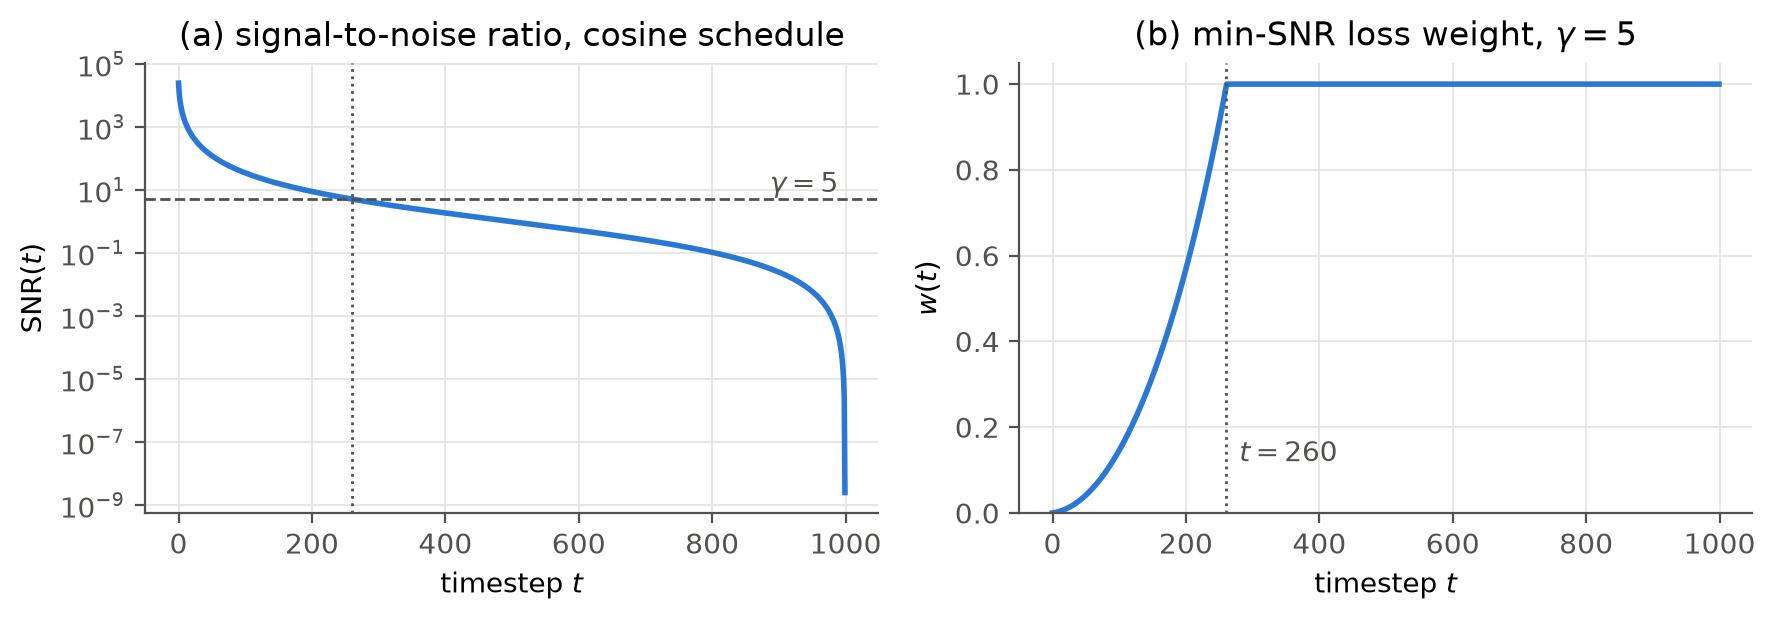
\includegraphics[width=\linewidth]{ext_minsnr_weight.png}
    \caption{(a) Signal-to-noise ratio of the noisy image under the clipped cosine schedule, with the
    cap $\gamma = 5$ dashed. (b) The resulting weight on the $\varepsilon$-prediction loss. Timesteps
    to the right of $t = 260$ are unaffected. Drawn from Equations~\eqref{eq:ext-snr}
    and~\eqref{eq:ext-minsnr}, following Hang et al.\ \parencite{arXiv:2303.09556}.}
    \label{fig:ext-minsnr}
\end{figure}

Hang et al.\ report that the weighting reaches a given FID several times sooner than the standard
objective, but their evidence comes from networks considerably larger than the 2.47
million-parameter network of rung E3. Its
effect at this scale is therefore not assumed; the rung measures it, and if the weighting does not
help, the result will show it.

\subsection{Five Times the Training (E4)}

E4 extends training from 30 to 150 epochs, or from 11\,700 to 58\,500 steps, and so reduces the
shortfall in optimisation steps against Ho et al.\ from a factor of 68 to one of 14. It is the most
direct response to the first cause and involves no change of method at all.

\subsection{Increased Capacity (E5)}

E5 widens the network and deepens each stage. On CIFAR-10 the widths change from $(64, 128)$ to
$(128, 256, 256)$ with two residual blocks per stage instead of one, which takes the parameter count
from 2.47 million to 31.46 million, $88\%$ of the 35.7 million of Ho et al. The widths and block
count follow the published configuration, whose base width is 128 with two residual blocks at each
resolution. On CelebA, which already has three stages, the widths change from $(32, 64, 128)$ to
$(96, 192, 256)$, taking the count from 2.61 million to 24.41 million.

E5 is trained for the same 150 epochs as E4, so the difference between them is due to capacity
alone. That capacity arrives in three forms at once on CIFAR-10, however: wider layers, a second
block per stage, and a third resolution stage. The rung therefore cannot serve as a test of the depth
hypothesis raised in Section~\ref{sec:distribution}, which requires the number of stages to change
while the width is held fixed.

\subsection{Long Training (E6)}
\label{sec:ext-long}

E6 spends the remainder of the available time on the E5 network. It resumes from the E5 checkpoint,
weights, optimiser state and moving average included, and continues to 2000 epochs on CIFAR-10 and
700 on CelebA. On CIFAR-10 this is 780\,000 optimisation steps, $97.5\%$ of the 800\,000 of Ho et
al., so the shortfall in steps that dominated the budget of Chapter~\ref{ch3} is essentially removed
(Table~\ref{tab:ext-budget}). A CelebA step costs 2.8 times as much as a CIFAR-10 step, and 700 epochs,
or 273\,000 steps, gives the two datasets roughly equal shares of the time.

\begin{table}[htbp]
    \centering
    \caption{Training budget of the extended rungs on CIFAR-10, continuing
    Table~\ref{tab:budget}. E6 removes the shortfall in optimisation steps; the remaining
    difference from the published configuration lies in the architecture.}
    \label{tab:ext-budget}
    \begin{tabular}{lrrrrr}
        \toprule
        & Chapter~\ref{ch3} & E4 & E5 & E6 & Ho et al. \\
        \midrule
        Parameters         & 2.47\,M & 2.47\,M & 31.46\,M & 31.46\,M & 35.7\,M \\
        Optimisation steps & 11\,700 & 58\,500 & 58\,500  & 780\,000 & 800\,000 \\
        Steps relative to Ho et al. & $1/68$ & $1/14$ & $1/14$ & $0.98$ & $1$ \\
        \bottomrule
    \end{tabular}
\end{table}

Resuming rather than starting afresh means that E5 is the 150-epoch point on the trajectory of E6,
not an independent run, and costs nothing beyond its evaluation. It also means that the difference
between them combines the length of training with the change of averaging cap discussed in
Section~\ref{sec:ext-ema}. What remains between E6 and the published configuration is the
architecture: the reference network has four resolution stages rather than three, self-attention at
$16 \times 16$, and a skip connection from every block (Section~\ref{sec:simulation}). Those
differences are deliberately left in place, since this chapter asks what training alone can achieve.

\section{Sampling}
\label{sec:ext-sampling}

Every rung is evaluated with the thousand-step ancestral sampler of Chapter~\ref{ch3}, so that E0
can be compared with the earlier result and every rung with every other. The final rung on each
dataset is evaluated a second time with the deterministic sampler of Song et al.\
\parencite{arXiv:2010.02502}. It visits a subsequence $\tau_1 > \tau_2 > \dots > \tau_S$ of the
timesteps and, with its stochasticity parameter set to zero, updates
\begin{equation}
    x_{\tau_{i+1}} = \sqrt{\bar\alpha_{\tau_{i+1}}}\;\hat{x}_0
    + \sqrt{1 - \bar\alpha_{\tau_{i+1}}}\;\varepsilon_\theta(x_{\tau_i}, \tau_i),
    \qquad
    \hat{x}_0 = \frac{x_{\tau_i} - \sqrt{1 - \bar\alpha_{\tau_i}}\,
    \varepsilon_\theta(x_{\tau_i}, \tau_i)}{\sqrt{\bar\alpha_{\tau_i}}},
    \label{eq:ext-ddim}
\end{equation}
with $\hat{x}_0$ clipped to $[-1, 1]$ as in the ancestral sampler and $\bar\alpha$ taken as one after
the last step, so that the final update returns $\hat{x}_0$ itself. With $S = 100$ evenly spaced
timesteps it is ten times cheaper than the ancestral sampler. It is reported as a separate row because
a change of sampler changes the FID, and mixing the two would break the comparison along the ladder.

\section{Computational Budget}
\label{sec:ext-budget}

The rungs were fitted to a fixed allowance of 72 hours on the machine of Table~\ref{tab:environment}.
Two engineering measures made that allowance go considerably further than the settings of
Chapter~\ref{ch3} would have allowed, and one of them proved to be a prerequisite rather than an
optimisation.

\subsection{Graph Compilation}

The network was compiled with the graph compiler of PyTorch~2 \parencite{ansel2024pytorch}, which
fuses sequences of elementwise operations such as group normalisation and activation into single
kernels. Like the mixed precision and memory layout of Chapter~\ref{ch3}, this changes the arithmetic
used to evaluate the model and not the model itself. Table~\ref{tab:ext-steptime} reports the
measured effect. On the three smaller networks compilation shortens each step by a factor of 1.6 to
2.0. A second measure, removing the transfer of the loss from the graphics card to the host at every
step so that the processor no longer waits for each step to finish before issuing the next, gained a
further $8\%$ on the smallest network and raised the utilisation of the card from $91\%$ to $97\%$.

\begin{table}[htbp]
    \centering
    \caption{Measured time per optimisation step at a batch size of 128, with the card otherwise
    idle. Eager execution corresponds to the settings of Chapter~\ref{ch3}; its value for the
    ResUNet on CIFAR-10 reproduces the $16.0$\,s per epoch of Table~\ref{tab:cost}.}
    \label{tab:ext-steptime}
    \begin{tabular}{llrrr}
        \toprule
        Dataset & Network & Eager & Compiled & Speed-up \\
        \midrule
        CIFAR-10 & 2.47\,M (E0--E4)  & $41.0$\,ms  & $21.7$\,ms  & $1.9\times$ \\
        CIFAR-10 & 31.46\,M (E5, E6) & $221$\,ms   & $141$\,ms   & $1.6\times$ \\
        CelebA   & 2.61\,M (E0)      & $84.1$\,ms  & $43.1$\,ms  & $2.0\times$ \\
        CelebA   & 24.41\,M (E5, E6) & $3465$\,ms  & $390$\,ms   & $8.9\times$ \\
        \bottomrule
    \end{tabular}
\end{table}

The last row is not a speed-up in the ordinary sense. Executed eagerly, the large CelebA network
requires $12.9$\,GB at its peak, more than the 12\,GB the card provides. The graphics driver does not
report this as an error but silently borrows system memory, and each step then spends most of its
time waiting on transfers: the step takes $3.5$ seconds and the power drawn by the card falls to 88\,W,
against 190\,W when it is computing. Compilation reduces the peak to $7.2$\,GB by not materialising
intermediate tensors that the fused kernels no longer need, and the network fits. Without it, the
700 epochs of E5 and E6 on CelebA would have taken more than 260 hours. The implementation caps the memory available to
the process at $90\%$ of the card, so that an overflow of this kind stops the run with an error
rather than slowing it unnoticed.

\subsection{Compiled Sampling}

The thousand steps of the reverse process were compiled in the same way and, in addition, recorded
as a replayable sequence of kernels, which removes the cost of launching each kernel individually.
This shortens sampling by a factor of 2.0 to 3.0, and the 2048 samples needed for the FID of the
small CIFAR-10 network take $1.5$ minutes instead of $3.8$. Compilation reorders floating-point
operations, so the samples are not bit-for-bit identical to those of eager execution even from the
same noise. Its effect on the measurement was checked directly on the E0 checkpoint: eager sampling
gives an FID of $89.57$ and an Inception Score of $4.649$, compiled sampling $90.97$ and $4.650$. The
difference of $1.4$ FID is less than a fifth of the smallest seed-to-seed standard deviation observed
in Chapter~\ref{ch3}, and since every rung is evaluated the same way it cannot affect
$\Delta\mathrm{FID}$.

\subsection{Schedule}

Table~\ref{tab:ext-schedule} gives the resulting schedule. Training accounts for 61 of the 63 hours,
and the four large-network rungs for $96\%$ of the total. The remaining nine hours of the allowance
are held in reserve against the slowing of a card run continuously for three days and against
interruptions; checkpoints are written after every epoch, so an interrupted run resumes where it
stopped.

\begin{table}[htbp]
    \centering
    \caption{Schedule of the complete ladder, computed from the measured step times of
    Table~\ref{tab:ext-steptime}. One epoch is 390 steps on both datasets.}
    \label{tab:ext-schedule}
    \begin{tabular}{lrrr}
        \toprule
        Item & Epochs & Seconds per epoch & Time \\
        \midrule
        CIFAR-10 E0--E3              & $4 \times 30$ & 8.5  & 17\,min \\
        CIFAR-10 E4                  & 150           & 8.5  & 21\,min \\
        CIFAR-10 E5                  & 150           & 55   & 2\,h 18\,min \\
        CIFAR-10 E6 (from E5)        & $+1850$       & 55   & 28\,h 16\,min \\
        CelebA E0                    & 30            & 16.8 & 8\,min \\
        CelebA E5                    & 150           & 152  & 6\,h 20\,min \\
        CelebA E6 (from E5)          & $+550$        & 152  & 23\,h 13\,min \\
        Compilation, once per rung   &               &      & 8\,min \\
        \midrule
        Training                     &               &      & 61\,h \\
        Evaluation and figures       &               &      & 1\,h 40\,min \\
        \midrule
        Total                        &               &      & 63\,h \\
        \bottomrule
    \end{tabular}
\end{table}

\section{Results}
\label{sec:ext-results}

\subsection{How the Results Are to Be Read}

The rules for interpreting the ladder are fixed here, before the results are known, so that they
cannot be chosen to suit them.

\begin{enumerate}
    \item \textbf{Only $\Delta\mathrm{FID}$ supports a causal claim.} The absolute FID of a rung
    includes the effect of every change above it.

    \item \textbf{Each rung is a single run.} Chapter~\ref{ch3} measured the seed-to-seed standard
    deviation of FID for this network at $21.13$ on CIFAR-10 and $23.98$ on CelebA. A rung whose
    $\Delta\mathrm{FID}$ is smaller in magnitude than that cannot be said to have had an effect, and
    will be reported as inconclusive rather than as a small improvement.

    \item \textbf{E0 must reproduce Chapter~\ref{ch3}.} The criterion is agreement with $94.93$ to
    within one standard deviation. The preliminary evaluation reported in Section~\ref{sec:ext-design}
    already meets it.

    \item \textbf{Bundled rungs are reported as bundles.} E2 is one result for three stabilisers,
    E5 one result for width, depth and a third stage on CIFAR-10, and E6 one result for training
    length and averaging cap together.
\end{enumerate}

\subsection{Measurements}

% 실행이 끝나면 model/extension/extension_study.json 에서 옮긴다.
% 키: "<데이터셋>|<단계>|ancestral" 과 "<데이터셋>|E6|ddim100"
% loss_final -> 손실, fid -> FID, is_mean -> IS. ΔFID 는 바로 위 행과의 차
\noindent\textit{The measurements below are completed from the output of the 72-hour run described
in Section~\ref{sec:ext-budget}. Epochs and parameter counts are fixed by the design and are given
in advance.}

\begin{table}[htbp]
    \centering
    \caption{Results of the ladder. $\Delta$FID is the difference from the row above and is the
    contribution of that rung. The final row of each dataset uses the deterministic sampler and is
    compared with the row above it.}
    \label{tab:ext-results}
    \small
    \begin{tabular}{llrrrrrr}
        \toprule
        Dataset & Rung & Epochs & Parameters & Final loss & FID & $\Delta$FID & IS \\
        \midrule
        CIFAR-10 & E0 & 30   & 2\,473\,475  & --- & --- & ---  & --- \\
        CIFAR-10 & E1 & 30   & 2\,473\,475  & --- & --- & ---  & --- \\
        CIFAR-10 & E2 & 30   & 2\,473\,475  & --- & --- & ---  & --- \\
        CIFAR-10 & E3 & 30   & 2\,473\,475  & --- & --- & ---  & --- \\
        CIFAR-10 & E4 & 150  & 2\,473\,475  & --- & --- & ---  & --- \\
        CIFAR-10 & E5 & 150  & 31\,460\,739 & --- & --- & ---  & --- \\
        CIFAR-10 & E6 & 2000 & 31\,460\,739 & --- & --- & ---  & --- \\
        CIFAR-10 & E6, deterministic, 100 steps & 2000 & 31\,460\,739 & & --- & --- & --- \\
        \midrule
        CelebA   & E0 & 30   & 2\,612\,419  & --- & --- & ---  & --- \\
        CelebA   & E5 & 150  & 24\,408\,291 & --- & --- & ---  & --- \\
        CelebA   & E6 & 700  & 24\,408\,291 & --- & --- & ---  & --- \\
        CelebA   & E6, deterministic, 100 steps & 700 & 24\,408\,291 & & --- & --- & --- \\
        \bottomrule
    \end{tabular}
\end{table}

\begin{figure}[htbp]
    \centering
    \IfFileExists{imgs/ext_fid_ladder.png}{%
        \includegraphics[width=\linewidth]{ext_fid_ladder.png}%
    }{%
        \fbox{\parbox[c][4cm][c]{0.9\linewidth}{\centering\itshape
        FID by rung; generated by Section 10 of the extension notebook}}%
    }
    \caption{FID at each rung, with the seed-0 ResUNet result of Chapter~\ref{ch3} dashed.}
    \label{fig:ext-fid-ladder}
\end{figure}

\begin{figure}[htbp]
    \centering
    \IfFileExists{imgs/ext_samples_cifar10.png}{%
        \includegraphics[width=\linewidth]{ext_samples_cifar10.png}%
    }{%
        \fbox{\parbox[c][3cm][c]{0.9\linewidth}{\centering\itshape
        CIFAR-10 samples by rung; generated by Section 10 of the extension notebook}}%
    }\\[3mm]
    \IfFileExists{imgs/ext_samples_celeba.png}{%
        \includegraphics[width=\linewidth]{ext_samples_celeba.png}%
    }{%
        \fbox{\parbox[c][3cm][c]{0.9\linewidth}{\centering\itshape
        CelebA samples by rung; generated by Section 10 of the extension notebook}}%
    }
    \caption{Samples from each rung on CIFAR-10 (top) and CelebA (bottom). Every panel starts from
    the same initial noise, so differences between panels are due to the training configuration
    alone.}
    \label{fig:ext-samples}
\end{figure}

\section{Limitations}
\label{sec:ext-limitations}

The most serious limitation is the one Chapter~\ref{ch3} was at pains to establish: a single run
cannot distinguish an effect from the seed-to-seed variation unless the effect is large. The
72-hour allowance was spent on length of training rather than on repetition, because the question
of this chapter concerns absolute quality, and the reading rules above are the price of that choice.

The ladder measures each change in the context of those above it. The moving average in particular
is likely to be worth more in a short run, where the final iterate is far from settled, than it would
be if added at the end of a long one; E1 measures it at thirty epochs and makes no claim beyond that.
Three rungs combine several changes, as set out in Section~\ref{sec:ext-rationale}.

The FID is again computed from 2048 samples, for comparability with Chapter~\ref{ch3}, and remains
biased upward at that size; the absolute values should not be compared with published figures computed
from fifty thousand. Compiled sampling introduces a numerical difference that was measured at
$1.4$~FID on one checkpoint.

Several remedies were deliberately left out because they would change the method rather than its
training. Predicting the velocity $v$ instead of the noise alters the implicit weighting across
timesteps and hence the regression to the mean discussed in Section~\ref{sec:ext-motivation}
\parencite{arXiv:2202.00512}. Classifier-free guidance is the most effective single remedy for
indistinct samples in current practice \parencite{arXiv:2207.12598}, but it requires a conditional
model and does not apply to the unconditional generation studied here. And the architectural
differences from the reference network, among them self-attention and a fourth resolution stage,
are left in place so that the result measures what training alone can achieve.

\section{Summary}

This chapter applies to the proposed network the remedies that Chapter~\ref{ch3} and the Conclusions
identified for its indistinct samples. Seven cumulative rungs add an average of the weights, three
training stabilisers, a reweighting of the loss across timesteps, five times the training, nearly
thirteen times the parameters and, finally, sixty-seven times the optimisation steps of the original
experiment, which brings the step count on CIFAR-10 to within $2.5\%$ of the published configuration.
The reasoning behind each change and the value chosen for it are set out in
Section~\ref{sec:ext-rationale}, and the rules by which the results are to be read are fixed in
Section~\ref{sec:ext-results} ahead of them.

Two findings are already in hand. The pipeline reproduces the seed-0 result of Chapter~\ref{ch3}
to within a quarter of a standard deviation, which validates every rung built on it. And graph
compilation is not merely an acceleration at this scale but a condition of the experiment: without
it the largest network does not fit in the memory of the card, and the driver's silent fallback to
system memory makes it nine times slower without reporting any fault.


\chapter*{Conclusions}
\addcontentsline{toc}{chapter}{Conclusions}
\label{Conclusions}

This project set out to determine whether combining residual learning with the UNet backbone
conventionally used as the denoising network of a diffusion model improves the quality of the images
it generates. A Denoising Diffusion Probabilistic Model was implemented from first principles and
the diffusion framework was held fixed while three denoising networks were substituted into it: the
proposed residual UNet, an otherwise identical network with the identity shortcut removed, and the
reference architecture of Ho et al.\ narrowed to a matching parameter budget. Each was trained on
CIFAR-10 at $32 \times 32$ and on CelebA at $64 \times 64$ under identical conditions.

\section*{Findings}

The answer to the question as posed is that residual learning helps, but conditionally, and not in
the way the project anticipated.

The shortcut makes optimisation easier at the outset. After one epoch the proposed network leads its
shortcut-free twin in all six paired runs, by $5.4\%$ on average on CIFAR-10 and $11.1\%$ on
CelebA, and since the two differ in nothing else the shortcut is the only possible cause. That
advantage is gone by the fifth epoch and does not reappear: at convergence the restoration measures
cannot separate the two networks, and the two that lean at all lean in opposite directions, the
training loss favouring the plain network and structural similarity the proposed one, both by less
than half of one per cent.

They are not, however, indistinguishable as generators, and repeating each configuration under three
seeds is what makes the distinction legible. On CelebA the proposed network leads in every seed, by
$59$, $22$ and $109$ Fréchet Inception Distance, for a mean advantage of $63.31$ against a
seed-to-seed standard deviation of about $23$ for either network. On CIFAR-10 the same comparison
yields $-3.46 \pm 13.78$ with the sign changing between seeds, which is to say no effect at all;
the apparent reversal seen in a single run was noise. The difference between the two datasets tracks
depth, the CelebA configuration having three resolution stages against two for CIFAR-10, and
residual connections exist precisely to make deeper networks optimisable. Where the network is
shallow enough not to need one, adding it changes nothing; where it is deep enough to struggle
without one, it is worth sixty points of FID.

The reference architecture remains the strongest network overall. It leads on every restoration
measure on both datasets and on CIFAR-10 FID by a wide margin, while using fewer parameters than
either competitor, at roughly $2.3$ times the training cost per epoch. Only on CelebA FID is it
matched, and there the proposed network achieves the same quality for less than half the compute.

Two results of a different kind emerged from the work and are worth recording. The first is
methodological: a network can denoise as well as another and generate images that are $78\%$ worse
by FID. The training objective averages the noise-prediction error uniformly over timesteps, whereas
generation composes a thousand such predictions in sequence, so errors that are small on average but
systematic at particular timesteps compound through that composition. Evaluating a diffusion model
by reconstruction alone is not sufficient. The second is practical: the algebraic form of the
posterior mean used in the reverse process is numerically stable only for a network whose noise
prediction is already accurate. Without clipping the implied estimate of $x_0$ at every step, the
reverse process diverged from a standard deviation of $1$ to approximately $16$, in single precision
as well as mixed, and produced saturated noise from every model.

\section*{Limitations}

Each configuration was trained three times. Three runs are enough to establish that a sign is
consistent and to estimate a standard deviation, but not to support a formal claim of significance:
the paired test on the CelebA result gives $t(2) = -2.50$, which does not reach the conventional
threshold with two degrees of freedom. The finding rests on the direction being the same in every
run and the magnitude exceeding the observed spread, not on a $p$-value. The depth explanation
offered for the difference between datasets is consistent with the evidence but not established by
it, since depth and resolution vary together here; separating them would require the two-stage and
three-stage configurations to be trained on the same images.

The seed study also showed that the Fréchet Inception Distance is far noisier at this scale than the
restoration measures, with standard deviations between $7.8$ and $32.9$ against thousandths for
SSIM. Any comparison of diffusion models drawn from a single training run of this length, including
several reported in the earlier sections of this work before the repetition was carried out, should
be treated with corresponding caution.

Thirty epochs amounts to roughly eleven thousand optimisation steps, some two orders of magnitude
short of the schedule used for the published CIFAR-10 configuration, and the networks are about
fourteen times smaller. The absolute FID values are correspondingly poor and should not be compared
with the literature; only the relative ordering between the three networks, which were trained
identically, carries meaning. The Fréchet Inception Distance was computed from two thousand samples,
which is the smallest number at which the estimate is not degenerate given the dimensionality of the
Inception feature space, and remains biased upward at that size.

One standard practice was omitted. Diffusion implementations customarily sample not from the trained weights themselves but from an exponential moving average of them, which suppresses the fluctuation of the final iterates and typically improves the Fr\'echet Inception Distance appreciably. No such average was maintained here, so the absolute sample quality reported is lower than the same training run would otherwise have produced. The omission applies identically to all six runs and so does not affect the comparison between them.

The memorisation check operates in pixel space and would not detect a reproduction that had been
shifted or recoloured. Negative Log-Likelihood was excluded on the grounds that this implementation
fixes the reverse-process variances rather than learning them. The comparison against Variational
Autoencoders and Generative Adversarial Networks set out in Chapter~\ref{ch2} was not carried out.

\section*{Further work}

The immediate priority is more repetition. Three seeds established which of the single-run findings
survive, but the surviving one is supported by consistency of sign rather than by a significance
test; ten seeds would permit a confidence interval, and at the cost of the deterministic sampler
described below would remain affordable.

The depth hypothesis is directly testable. Training two-stage, three-stage and four-stage variants
of the proposed network on a single dataset, each with and without the shortcut, would isolate depth
from resolution and determine whether the benefit of residual learning grows with the former as the
argument predicts.

A separate line of work concerns the absolute quality of the samples rather than the comparison between architectures. Three changes would address it, in descending order of expected effect and ascending order of cost. Maintaining an exponential moving average of the weights and sampling from it is the cheapest, requiring a few lines and no change to the experimental design. Extending training by an order of magnitude is the most certain, since Section~\ref{sec:indistinct} attributes the indistinctness principally to the budget. Replacing the ancestral sampler with the deterministic variant of Song et al.\ would allow comparable quality from roughly fifty reverse steps instead of a thousand, which would also reduce the cost of computing the Fr\'echet Inception Distance by a factor of twenty and so make the repeated runs recommended above considerably cheaper. None of the three alters the architectures under test, so each could be applied to all six configurations without disturbing the comparison.

Beyond that, learning the reverse-process variances rather than fixing them would make the
variational bound informative and bring Negative Log-Likelihood within reach, and the Variational
Autoencoder and Generative Adversarial Network baselines would place the diffusion results in the
wider context that Chapter~\ref{ch2} describes but does not measure.


% 부록: \appendix 를 켜야 "Appendix A" 로 번호가 매겨짐
\appendix
\chapter{Appendices}
\label{appendix}

\section{Per-Epoch Training Loss}
\label{sec:loss-full}

Table~\ref{tab:loss} in Chapter~\ref{ch3} reports the training loss at five checkpoints.
Table~\ref{tab:loss-full} gives the complete record for the six runs under seed 0, so that the shape
of the curves discussed in Section~\ref{sec:convergence} can be inspected directly. The other two
seeds follow the same trajectory and are not reproduced; their final values appear in
Table~\ref{tab:fid} and the underlying record is available in the accompanying repository.

The epoch at which one network overtakes another is not itself stable across seeds, and
Table~\ref{tab:crossover} records where it falls. The proposed network is overtaken by its
shortcut-free variant somewhere between the third and the sixth epoch on both datasets, which is
consistent with the early advantage being real but short-lived. The reference network is more
erratic: on CIFAR-10 it takes the lead as early as the second epoch under one seed and as late as
the twelfth under another, although it finishes ahead in every case. These figures are a further
reminder that quantities read from a single run should not be quoted to a precision the experiment
does not support.

\begin{table}[htbp]
    \centering
    \caption{The epoch at which one network first attains a lower training loss than another.}
    \label{tab:crossover}
    \small
    \begin{tabular}{llccc}
        \toprule
        Comparison & Dataset & Seed 0 & Seed 1 & Seed 2 \\
        \midrule
        plain overtakes ResUNet & CIFAR-10 & 4 & 4 & 3 \\
        plain overtakes ResUNet & CelebA   & 5 & 3 & 6 \\
        \midrule
        DDPM UNet leads both    & CIFAR-10 & 11 & 2 & 12 \\
        DDPM UNet leads both    & CelebA   & 2 & 1 & 2 \\
        \bottomrule
    \end{tabular}
\end{table}

\begin{table}[htbp]
    \centering
    \caption{Epoch-averaged noise-prediction loss for the six runs under seed 0. Lower is better.}
    \label{tab:loss-full}
    \footnotesize
    \begin{tabular}{ccccccc}
        \toprule
        & \multicolumn{3}{c}{CIFAR-10} & \multicolumn{3}{c}{CelebA} \\
        \cmidrule(lr){2-4} \cmidrule(lr){5-7}
        Epoch & ResUNet & plain & DDPM UNet & ResUNet & plain & DDPM UNet \\
        \midrule
        1 & 0.13775 & 0.14633 & 0.18508 & 0.14205 & 0.16413 & 0.15588 \\
        2 & 0.08237 & 0.08327 & 0.08805 & 0.06335 & 0.06774 & 0.06071 \\
        3 & 0.07665 & 0.07676 & 0.07861 & 0.05415 & 0.05513 & 0.04980 \\
        4 & 0.07322 & 0.07265 & 0.07399 & 0.04957 & 0.04963 & 0.04503 \\
        5 & 0.07111 & 0.07033 & 0.07135 & 0.04735 & 0.04705 & 0.04316 \\
        6 & 0.07017 & 0.06936 & 0.07014 & 0.04535 & 0.04496 & 0.04136 \\
        7 & 0.06790 & 0.06719 & 0.06799 & 0.04430 & 0.04379 & 0.04057 \\
        8 & 0.06705 & 0.06637 & 0.06672 & 0.04283 & 0.04234 & 0.03927 \\
        9 & 0.06655 & 0.06582 & 0.06591 & 0.04207 & 0.04159 & 0.03863 \\
        10 & 0.06619 & 0.06555 & 0.06593 & 0.04110 & 0.04055 & 0.03779 \\
        11 & 0.06570 & 0.06511 & 0.06491 & 0.04094 & 0.04044 & 0.03761 \\
        12 & 0.06517 & 0.06455 & 0.06448 & 0.03977 & 0.03924 & 0.03665 \\
        13 & 0.06458 & 0.06409 & 0.06386 & 0.03994 & 0.03948 & 0.03699 \\
        14 & 0.06424 & 0.06365 & 0.06360 & 0.03984 & 0.03935 & 0.03677 \\
        15 & 0.06424 & 0.06373 & 0.06322 & 0.03915 & 0.03866 & 0.03639 \\
        16 & 0.06352 & 0.06308 & 0.06281 & 0.03938 & 0.03891 & 0.03647 \\
        17 & 0.06315 & 0.06275 & 0.06206 & 0.03904 & 0.03855 & 0.03610 \\
        18 & 0.06305 & 0.06264 & 0.06202 & 0.03822 & 0.03775 & 0.03549 \\
        19 & 0.06278 & 0.06236 & 0.06196 & 0.03821 & 0.03773 & 0.03546 \\
        20 & 0.06249 & 0.06212 & 0.06165 & 0.03844 & 0.03799 & 0.03573 \\
        21 & 0.06250 & 0.06213 & 0.06158 & 0.03818 & 0.03772 & 0.03561 \\
        22 & 0.06265 & 0.06235 & 0.06160 & 0.03771 & 0.03727 & 0.03505 \\
        23 & 0.06170 & 0.06142 & 0.06062 & 0.03749 & 0.03712 & 0.03502 \\
        24 & 0.06204 & 0.06165 & 0.06080 & 0.03741 & 0.03700 & 0.03489 \\
        25 & 0.06218 & 0.06187 & 0.06091 & 0.03775 & 0.03726 & 0.03519 \\
        26 & 0.06132 & 0.06108 & 0.06040 & 0.03740 & 0.03704 & 0.03495 \\
        27 & 0.06156 & 0.06128 & 0.06075 & 0.03700 & 0.03659 & 0.03452 \\
        28 & 0.06190 & 0.06161 & 0.06071 & 0.03668 & 0.03626 & 0.03422 \\
        29 & 0.06165 & 0.06140 & 0.06059 & 0.03741 & 0.03700 & 0.03496 \\
        30 & 0.06108 & 0.06084 & 0.05967 & 0.03716 & 0.03679 & 0.03476 \\
        \bottomrule
    \end{tabular}
\end{table}

\section{Network Specifications}
\label{sec:specs}

The comparison in this work rests on the claim that the proposed and plain networks are identical in
size and that the reference network is comparable. Tables~\ref{tab:spec-resunet} and
\ref{tab:spec-ddpm} give the breakdown from which that claim can be checked.

The proposed and shortcut-free networks share every table entry, because an identity shortcut
introduces no parameters. Only the presence of the addition $x + h$ at the end of each block
differs, which is why the two rows of Table~\ref{tab:params} are equal to the digit.

\begin{table}[htbp]
    \centering
    \caption{Residual UNet, by stage. The figures apply unchanged to the shortcut-free variant.
    Each decoder concatenates the encoder features of the corresponding stage, so its block operates
    on the sum of the upsampled and skipped channel counts.}
    \label{tab:spec-resunet}
    \small
    \begin{tabular}{lccr}
        \toprule
        Stage & Channels & Resolution & Parameters \\
        \midrule
        \multicolumn{4}{l}{\emph{CIFAR-10, two resolution stages}} \\
        Timestep embedding MLP & --- & --- & 33\,024 \\
        Encoder 1 & $3 \rightarrow 64$ & $32 \times 32$ & 84\,160 \\
        Encoder 2 & $64 \rightarrow 128$ & $16 \times 16$ & 386\,048 \\
        Bridge & $128$ & $8 \times 8$ & 312\,192 \\
        Decoder 2 & $\rightarrow 256$ & $16 \times 16$ & 1\,279\,872 \\
        Decoder 1 & $\rightarrow 128$ & $32 \times 32$ & 377\,792 \\
        Final $1 \times 1$ convolution & $\rightarrow 3$ & $32 \times 32$ & 387 \\
        \emph{Total} & & & \emph{2\,473\,475} \\
        \midrule
        \multicolumn{4}{l}{\emph{CelebA, three resolution stages}} \\
        Timestep embedding MLP & --- & --- & 33\,024 \\
        Encoder 1 & $3 \rightarrow 32$ & $64 \times 64$ & 23\,648 \\
        Encoder 2 & $32 \rightarrow 64$ & $32 \times 32$ & 100\,864 \\
        Encoder 3 & $64 \rightarrow 128$ & $16 \times 16$ & 386\,048 \\
        Bridge & $128$ & $8 \times 8$ & 312\,192 \\
        Decoder 3 & $\rightarrow 256$ & $16 \times 16$ & 1\,279\,872 \\
        Decoder 2 & $\rightarrow 128$ & $32 \times 32$ & 377\,792 \\
        Decoder 1 & $\rightarrow 64$ & $64 \times 64$ & 98\,784 \\
        Final $1 \times 1$ convolution & $\rightarrow 3$ & $64 \times 64$ & 195 \\
        \emph{Total} & & & \emph{2\,612\,419} \\
        \bottomrule
    \end{tabular}
\end{table}

Two features of Table~\ref{tab:spec-resunet} are worth noting. The first is that the coarsest
decoder dominates the budget, holding $52\%$ of the parameters on CIFAR-10 and $49\%$ on CelebA,
because concatenation doubles the channel count before the block that follows it. The second is that
adding a third resolution stage for CelebA increases the total by only $5.6\%$: the channel widths
were narrowed from $(64, 128)$ to $(32, 64, 128)$ so that the deeper network would remain comparable
in size to the shallower one, which is what permits the two datasets to be discussed on the same
footing.

\begin{table}[htbp]
    \centering
    \caption{Reference DDPM UNet, by functional group. The same configuration is used for both
    datasets, since none of its parameter counts depends on the input resolution.}
    \label{tab:spec-ddpm}
    \small
    \begin{tabular}{lr}
        \toprule
        Group & Parameters \\
        \midrule
        Timestep embedding MLP & 131\,712 \\
        Input convolution & 896 \\
        Downward residual blocks (8) & 523\,328 \\
        Downward attention & 33\,536 \\
        Downsampling convolutions (3) & 83\,104 \\
        Middle block (residual, attention, residual) & 181\,504 \\
        Upward residual blocks (12) & 1\,240\,640 \\
        Upward attention & 50\,304 \\
        Upsampling convolutions (3) & 110\,784 \\
        Output normalisation and convolution & 931 \\
        \midrule
        \emph{Total} & \emph{2\,356\,739} \\
        \bottomrule
    \end{tabular}
\end{table}

The reference network reaches a similar total by a different distribution. Its upward path carries
$53\%$ of the parameters, because a skip connection is taken from every residual block rather than
once per resolution stage, so each of the twelve upward blocks receives a concatenated input. The
attention layers account for only $3.6\%$ of the weights while contributing a large share of the
runtime, which is why this network costs roughly $2.3$ times as much per epoch despite being the
smallest of the three.

\section{Memorisation Check: Remaining Configurations}
\label{sec:memo-full}

Figure~\ref{fig:memorisation} in Chapter~\ref{ch3} shows the closest generated and training pairs
for the proposed network on CelebA. The remaining five configurations are given here, and support
the same conclusion: in no case is a generated sample a reproduction of a training image.

\begin{figure}[htbp]
    \centering
    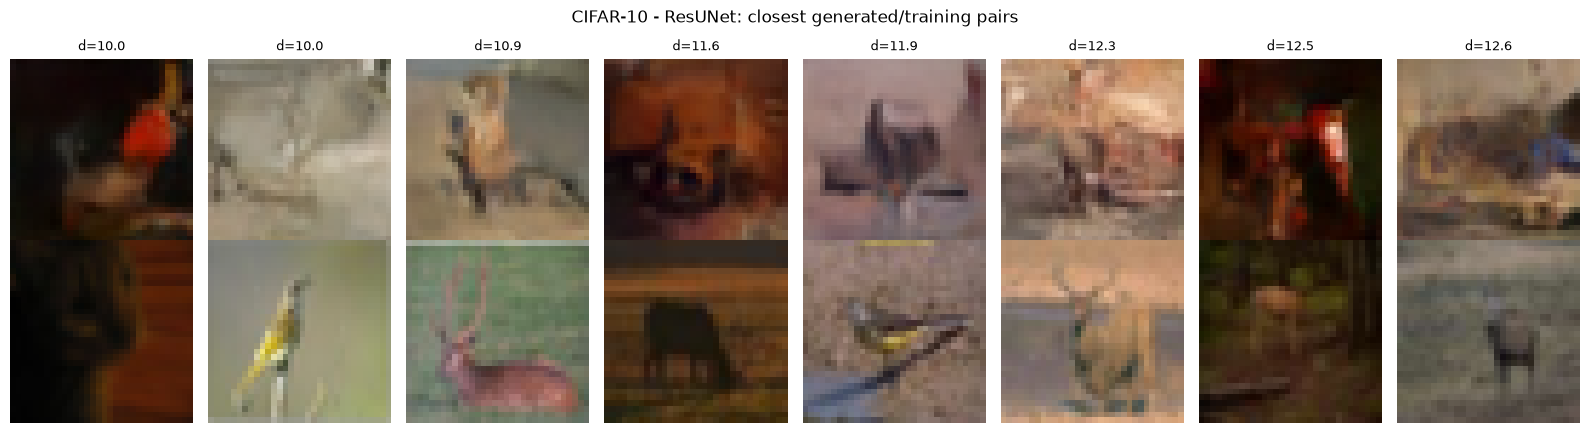
\includegraphics[width=\linewidth]{memo_cifar10_resunet.png}\\[2mm]
    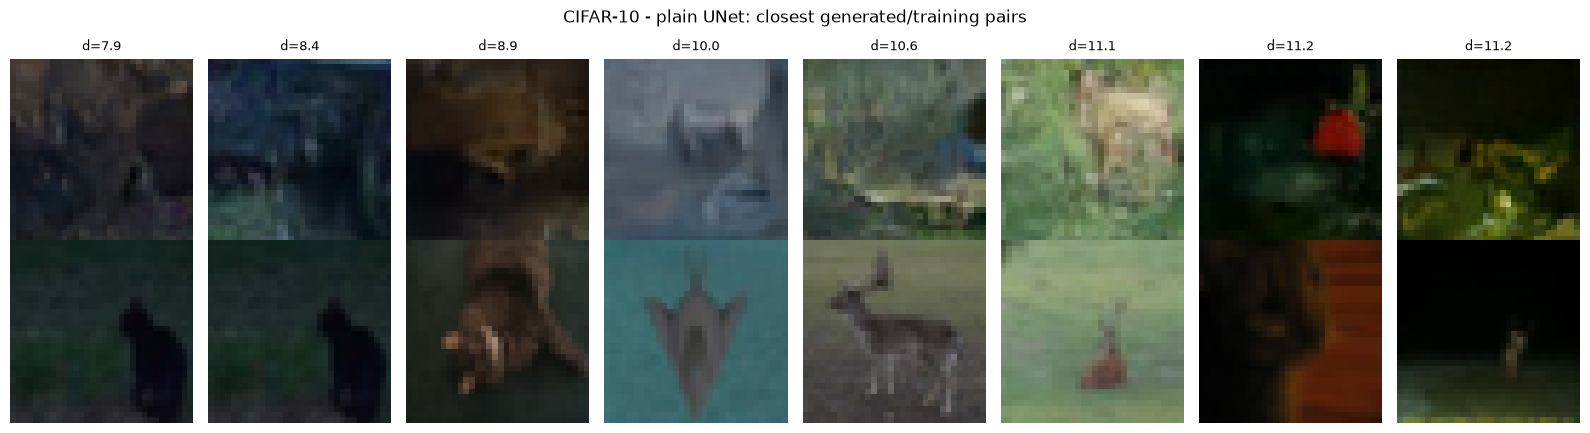
\includegraphics[width=\linewidth]{memo_cifar10_plain.png}\\[2mm]
    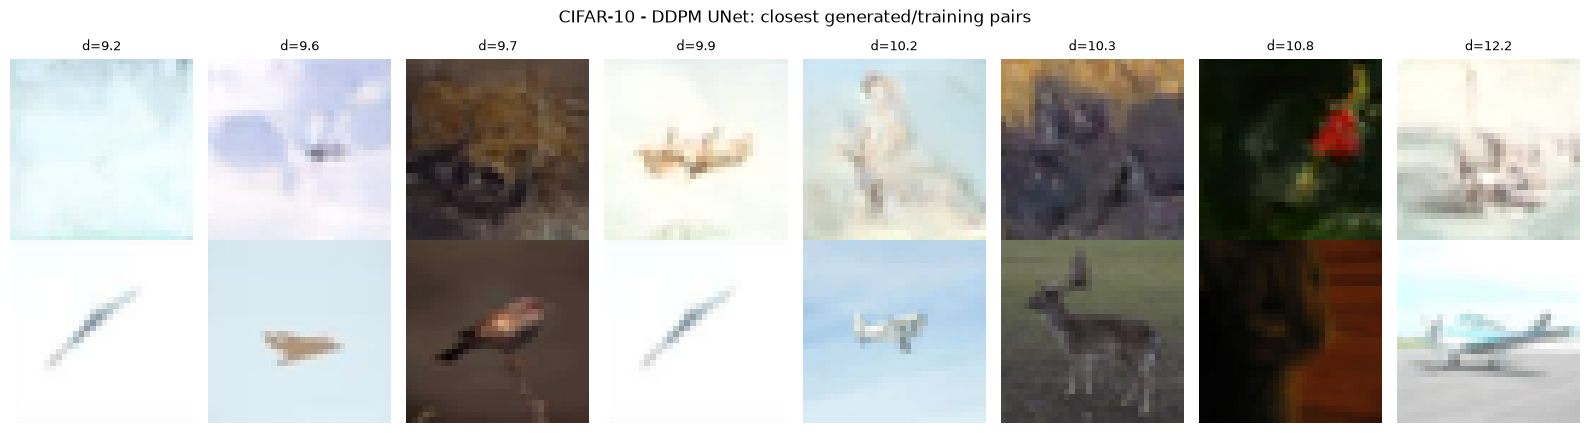
\includegraphics[width=\linewidth]{memo_cifar10_ddpm.png}
    \caption{CIFAR-10: the eight samples closest to the training set (top row of each pair) with
    their nearest training image (bottom row), for the proposed, shortcut-free and reference
    networks in turn.}
    \label{fig:memo-cifar}
\end{figure}

\begin{figure}[htbp]
    \centering
    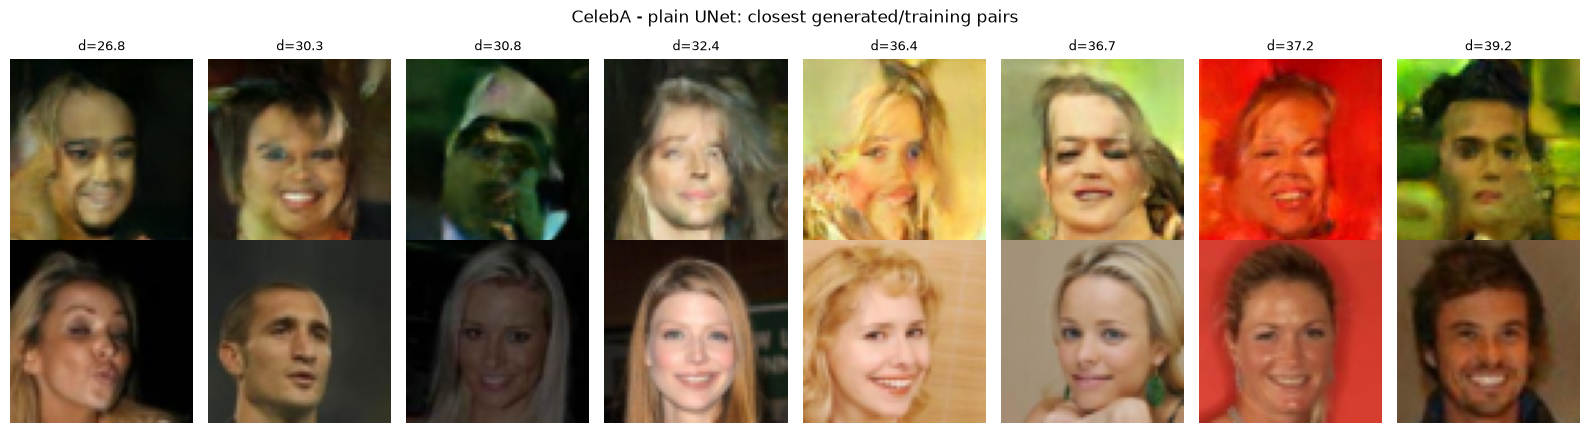
\includegraphics[width=\linewidth]{memo_celeba_plain.png}\\[3mm]
    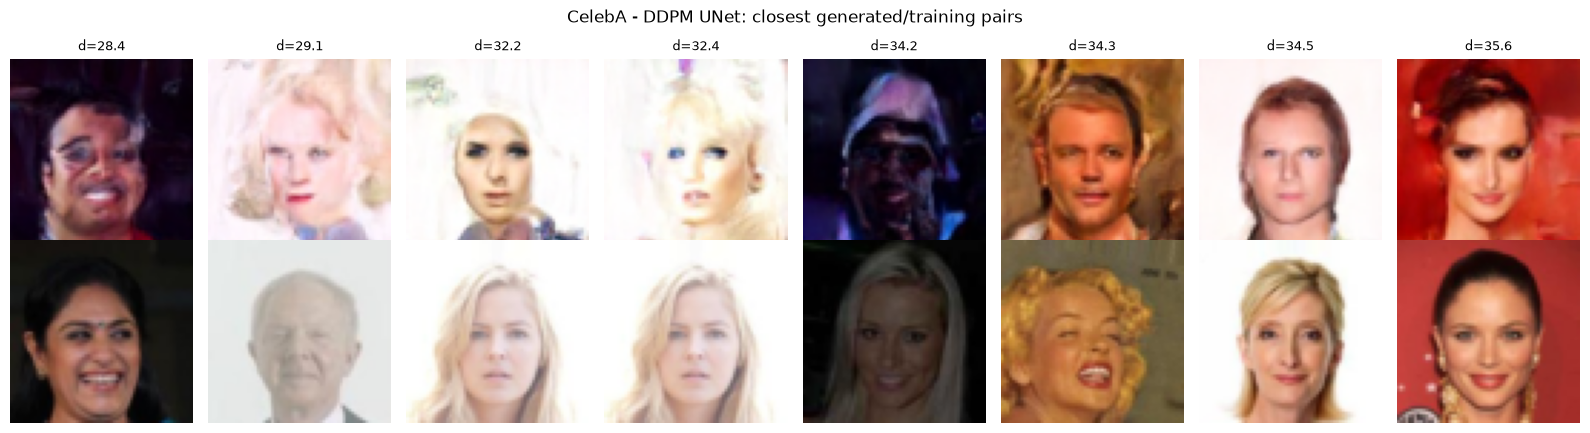
\includegraphics[width=\linewidth]{memo_celeba_ddpm.png}
    \caption{CelebA: the shortcut-free and reference networks. No pair depicts the same person.}
    \label{fig:memo-celeba}
\end{figure}

\section{Computing Environment}
\label{sec:environment}

All eighteen runs were carried out on the machine described in Table~\ref{tab:environment}. Six
configurations trained for thirty epochs under each of three seeds amount to approximately five
hours of training, and the evaluation adds a further two and a half, dominated by drawing the two
thousand samples per model required for the Fr\'echet Inception Distance. The complete experiment
therefore occupies about seven and a half hours on a single consumer graphics card, which is what
makes the repetition recommended in the Conclusions practical rather than aspirational.

\begin{table}[htbp]
    \centering
    \caption{Hardware and software used for every run reported in this work.}
    \label{tab:environment}
    \small
    \begin{tabular}{ll}
        \toprule
        Component & Version \\
        \midrule
        GPU & NVIDIA GeForce RTX 4070, 12\,GB \\
        Driver & 591.86 \\
        Operating system & Windows 11 \\
        Python & 3.12.10 \\
        PyTorch & 2.14.0+cu130 \\
        torchvision & 0.29.0+cu130 \\
        CUDA runtime & 13.0 \\
        cuDNN & 9.24.0 \\
        torchmetrics & 1.9.0 \\
        torch-fidelity & 0.4.0 \\
        scikit-image & 0.26.0 \\
        NumPy & 2.5.2 \\
        \bottomrule
    \end{tabular}
\end{table}

Training used bfloat16 mixed precision with the channels-last memory format, and TF32 matrix
multiplication with the cuDNN autotuner enabled. These settings affect only the arithmetic used to
evaluate a fixed model, not the model itself, and were applied identically to all six runs.

The implementation is a single Jupyter notebook containing the network definitions, the diffusion
process, the training loop and every evaluation reported here. It includes a self-check routine that
verifies the noise schedule is monotone and converges to the standard normal distribution, that the
closed-form forward process is consistent, that the network output depends on the timestep, that the
sampling path executes, and that the parameter budgets of the three architectures satisfy the
constraints stated in Section~\ref{sec:simulation}. Datasets are decoded once into unsigned
eight-bit tensors and cached, so that only the first execution pays the preprocessing cost, and
training is skipped for any architecture whose checkpoint already records the full number of epochs.


\printbibliography[title={References},heading=bibintoc]

\end{document}
